\documentclass[uplatex, dvipdfmx]{jsreport}

% ============================================================
%  preamble.tex — 日本語数学ノート テンプレート共通設定
%
%  定理環境のカウンタ規約は tools/site が再現している：
%    - 全定理環境が definition のカウンタを共有（use counter from）
%    - カウンタは節ごとにリセット（number within=section）
%  この規約を変えるときは tools/site/lib/tex2md.mjs の
%  buildNumberMap() も合わせること（PDF とサイトで番号がずれる）。
% ============================================================

% --- 基本パッケージ ---
\usepackage{amsmath,amssymb,amsthm,mathtools}
\usepackage[dvipdfmx,hidelinks]{hyperref}
\usepackage{pxjahyper}

% --- 図・表 ---
\usepackage{tikz}
\usepackage{float}
\usetikzlibrary{decorations.pathreplacing,calc,arrows.meta,patterns,positioning}
\usepackage{pgfplots}
\pgfplotsset{compat=1.18}
\usepackage{graphicx}
\graphicspath{{fig/}}

% --- 定理環境 (tcolorbox) ---
% 第 2 引数はラベル接頭辞。tools/site はこの接頭辞で \ref を解決するので、
% def / prop / thm / clm / lem / cor / rem / ex は変えないこと。
\usepackage{tcolorbox}
\tcbuselibrary{theorems,breakable}

% Definition: 青系
\newtcbtheorem[number within=section]{problem}{問題}{
  colback=teal!4, colframe=teal!55!black, fonttitle=\bfseries, breakable
}{prob}
% Definition: 青系
\newtcbtheorem[number within=section]{definition}{Def.}{
  colback=blue!5, colframe=blue!40!black, fonttitle=\bfseries, breakable
}{def}
% Proposition: オレンジ系
\newtcbtheorem[use counter from=definition]{proposition}{Prop.}{
  colback=orange!5, colframe=orange!50!black, fonttitle=\bfseries, breakable
}{prop}
% Theorem: 赤系（章・節の目玉となる重要結果）
\newtcbtheorem[use counter from=definition]{theorem}{Thm.}{
  colback=red!5, colframe=red!40!black, fonttitle=\bfseries, breakable
}{thm}
% Claim: 緑系（Thm ほど深くはないが，証明を要する主張）
\newtcbtheorem[use counter from=definition]{claim}{Claim}{
  colback=green!5, colframe=green!45!black, fonttitle=\bfseries, breakable
}{clm}
% Lemma: シアン系（命題の証明に用いる補助結果）
\newtcbtheorem[use counter from=definition]{lemma}{Lem.}{
  colback=cyan!5, colframe=cyan!50!black, fonttitle=\bfseries, breakable
}{lem}
% Corollary: すみれ系（定理から直ちに従う結果）
\newtcbtheorem[use counter from=definition]{corollary}{Cor.}{
  colback=violet!5, colframe=violet!40!black, fonttitle=\bfseries, breakable
}{cor}
% Remark: 黄系
\newtcbtheorem[use counter from=definition]{remark}{Rem.}{
  colback=yellow!5, colframe=yellow!40!black, fonttitle=\bfseries, breakable
}{rem}
% Example: 灰色系
\newtcbtheorem[use counter from=definition]{example}{Ex.}{
  colback=gray!5, colframe=gray!50!black, fonttitle=\bfseries, breakable
}{ex}
% Memo: 薄い黒系（番号なし，発展的補足）
\newtcolorbox{memo*}{
  colback=black!7, colframe=black!40,
  fonttitle=\bfseries, title={Memo},
  breakable
}
% 証明の直後が enumerate でも、最初の項目だけ見出しの横へずれないようにする。
% 通常の文章で始まる証明は従来どおり見出しと同じ行から始まる。
\makeatletter
\renewenvironment{proof}[1][\proofname]{\par
  \pushQED{\qed}%
  \normalfont \topsep6\p@\@plus6\p@\relax
  \trivlist
  \item[\hskip\labelsep\itshape #1\@addpunct{.}]\ignorespaces\leavevmode
}{%
  \popQED\endtrivlist\@endpefalse
}
\makeatother

% 証明環境の装飾
\tcolorboxenvironment{proof}{
  colback=white, colframe=black!20,
  leftrule=2pt, rightrule=0pt, toprule=0pt, bottomrule=0pt,
  breakable
}

% --- アルゴリズム環境 ---
\newcounter{algcounter}[section]
\newtcolorbox{algorithm}[1]{
  colback=white, colframe=black!70,
  fonttitle=\bfseries,
  title={Algorithm~\refstepcounter{algcounter}\thealgcounter\label{#1}},
  boxrule=0.8pt
}

% --- サイト向けの指示マクロ（PDF では何も出力しない）---
% \demohint{名前}: site.config.mjs の demos に登録した図をサイト側で差し込む
\newcommand{\demohint}[1]{}
% \blockmeta{...}: ブロックの機械可読メタデータ。PDF にもサイトにも出さない
\newcommand{\blockmeta}[1]{}

% ============================================================
%  数式マクロ
%  ここに書いたものは tools/site が自動抽出して MathJax にも渡す。
%  サイト側の設定に書き写す必要はない。
%  MathJax が解釈できない綴りだけ site.config.mjs の macroOverrides で
%  差し替えること（例: stmaryrd の \llbracket）。
% ============================================================

\newcommand{\R}{\mathbb{R}}
\newcommand{\N}{\mathbb{N}}
\newcommand{\Z}{\mathbb{Z}}
\newcommand{\Q}{\mathbb{Q}}
\newcommand{\E}{\mathbb{E}}

\newcommand{\X}{\mathcal{X}}
\newcommand{\Y}{\mathcal{Y}}
\newcommand{\Bb}{\mathcal{B}}
\newcommand{\Prob}{\mathcal{P}}

\DeclareMathOperator*{\argmin}{arg\,min}
\DeclareMathOperator*{\argmax}{arg\,max}
\DeclareMathOperator{\diag}{diag}
\DeclareMathOperator{\tr}{tr}
\DeclareMathOperator{\supp}{supp}
\DeclareMathOperator{\Id}{Id}

\newcommand{\abs}[1]{\lvert #1 \rvert}
\newcommand{\norm}[1]{\lVert #1 \rVert}
\newcommand{\inner}[2]{\langle #1,\, #2 \rangle}
\newcommand{\defeq}{\overset{\mathrm{def}}{=}}
\renewcommand{\d}{\mathrm{d}}

% --- 参考文献 ---
\usepackage[numbers,sort&compress]{natbib}


\renewcommand{\proofname}{証明}

\title{熊本大学 数学系大学院 入試\\{\Large 専門基礎科目のための教科書}}
\author{}
\date{\today}

\begin{document}
\maketitle

\begin{memo*}
専門基礎科目の過去問31題と予想問題3題を解くために必要な知識を、
前提から順に積み上げてまとめた一冊である。
$\sec$ の定義のような約束事から、行列式・固有値・コンパクト性まで、
「知らなければ手が止まる」ことを省略せずに収めた。

解答編（過去問・予想問題）が「その問題をどう解くか」を書くのに対し、
本書は「解く前に何を知っていればよいか」を書く。
定義と公式は暗記の対象なので、\textbf{覚える}と明記した箇所は結論を丸ごと記憶してよい。
一方、\textbf{導出}と書いた箇所は、記憶が飛んでも試験場で復元できるように筋道を示した。
\end{memo*}

\tableofcontents

\chapter{この本の使い方と記号}
\label{ch:tb-guide}

\section{何を収めたか}

専門基礎科目は、収録した5年度すべてで
\textbf{線形代数}・\textbf{微分積分}・\textbf{位相／距離空間}の三分野から出題されている。
本書はその三分野を、次の順に積み上げる。

\begin{enumerate}
  \item 第\ref{ch:tb-foundations}章：論理・集合・写像・実数・数列。三分野すべての土台。
  \item 第\ref{ch:tb-functions}章：初等関数と暗記すべき公式。$\sec$ や双曲線関数の約束もここ。
  \item 第\ref{ch:tb-differential}章・第\ref{ch:tb-integral}章：一変数の微分と積分。
  \item 第\ref{ch:tb-multivariable}章：多変数の微分積分。重積分、変数変換、Gamma・Beta 関数。
  \item 第\ref{ch:tb-linear-one}章・第\ref{ch:tb-linear-two}章：線形代数。空間と行列式、固有値と内積。
  \item 第\ref{ch:tb-topology}章：距離空間と位相空間。コンパクト性と連結性。
\end{enumerate}

各節の終わりには \textbf{Memo} を置き、その道具が過去問のどこで実際に使われたかを示した。
問題番号は解答編の表記（例：2021年度 第1期 専門基礎 第2問）に合わせている。

\section{読み方の約束}

\begin{itemize}
  \item \textbf{Def.}（定義）は言葉の意味を定める。定義は証明の対象ではなく、覚えて使うものである。
  \item \textbf{Thm.}（定理）・\textbf{Prop.}（命題）は証明できる主張である。
        入試で「示せ」と問われうるものには証明または導出の筋を付けた。
  \item \textbf{Ex.}（例）は、定義や定理が具体的にどう動くかを見る場所である。
  \item \textbf{Rem.}（注意）は、間違えやすい点をまとめた。
\end{itemize}

証明を省いた定理は、答案で「$\sim$ の定理より」と名前を挙げて引用してよいものに限った。
逆に、答案で結論だけ書くと減点されうる箇所には、そのつど注意を書いた。

\section{本書で使う記号}

\begin{definition}{数の集合と論理記号}{tb-notation-sets}
\[
\N=\{1,2,3,\ldots\},\quad
\Z=\{\ldots,-1,0,1,\ldots\},\quad
\Q,\quad \R,\quad \mathbb C
\]
をそれぞれ自然数、整数、有理数、実数、複素数の全体とする。
本書では $0\notin\N$ とし、$0$ を含めたいときは $n\ge0$ と書く。

論理記号は次の意味で使う。
\[
\forall\ \text{（任意の）},\quad
\exists\ \text{（ある〜が存在して）},\quad
\Longrightarrow\ \text{（ならば）},\quad
\Longleftrightarrow\ \text{（同値）}.
\]
$A\setminus B=\{x\in A\mid x\notin B\}$ を差集合、$A\sqcup B$ を
$A\cap B=\varnothing$ が分かっているときの合併（直和）とする。
\end{definition}

\begin{definition}{よく使う記法}{tb-notation-misc}
\[
\abs{x}\ \text{（絶対値）},\quad
\norm{x}\ \text{（ノルム）},\quad
\inner{x}{y}\ \text{（内積）},\quad
\lfloor x\rfloor\ \text{（床関数）}
\]
とする。行列 $A$ の行列式は $|A|$、転置は $A^{\mathsf T}$、
複素共役転置（随伴）は $A^{*}$ と書く。
$I_n$ は $n$ 次単位行列、$O$ は零行列、$\diag(d_1,\ldots,d_n)$ は対角行列である。
写像 $f$ の像を $f(A)$、逆像を $f^{-1}(B)$ と書く。
$f^{-1}$ は逆写像を意味するとは限らないことに注意する。
\end{definition}

\begin{remark}{$\R$ 上の区間}{tb-notation-interval}
\[
(a,b)=\{x\mid a<x<b\},\qquad
[a,b]=\{x\mid a\le x\le b\}
\]
とし、半開区間も同様に書く。$(a,b)$ は座標の組と同じ記号になるが、
文脈で区別する。曖昧になる場面では「開区間 $(a,b)$」と明示する。
\end{remark}

\begin{memo*}
答案で記号を使うときは、問題文で定義されていない記号を断りなく使わないこと。
$\sec$、$\operatorname{adj}$、$\Pi_k$ のような記号は、初出時に一行で定義を書いてから使う。
\end{memo*}

\chapter{論理・集合・写像・実数}
\label{ch:tb-foundations}

線形代数も微分積分も位相も、この章の言葉で書かれている。
特に「量化記号の順序」と「上限・下限」は、専門基礎の証明問題で毎年のように問われる。

\section{証明の型}

\begin{definition}{対偶・逆・裏}{tb-contraposition}
命題「$P\Longrightarrow Q$」に対し
\[
\text{対偶：}\ \lnot Q\Longrightarrow\lnot P,\qquad
\text{逆：}\ Q\Longrightarrow P,\qquad
\text{裏：}\ \lnot P\Longrightarrow\lnot Q
\]
という。ここで $\lnot P$ は $P$ の否定である。
\end{definition}

\begin{proposition}{対偶の同値性}{tb-contraposition-equiv}
$P\Longrightarrow Q$ と、その対偶 $\lnot Q\Longrightarrow\lnot P$ は同値である。
一方、逆と裏は元の命題と同値とは限らない。
\end{proposition}

\begin{remark}{証明の三つの型}{tb-proof-styles}
入試で使う型はほぼ次の三つに尽きる。
\begin{enumerate}
  \item \textbf{直接証明}：仮定から結論へ、定義と定理をつないで進む。
  \item \textbf{対偶証明}：結論の否定から仮定の否定を導く。
        「〜でないなら〜でない」の形の方が扱いやすいときに使う。
  \item \textbf{背理法}：結論の否定を仮定して矛盾を導く。
        「存在しない」「一意である」「無理数である」を示すときに有効である。
\end{enumerate}
また「反例を挙げよ」と問われたら、\textbf{仮定をすべて満たし結論だけが破れる}
具体例を一つ作ればよい。一般論を述べる必要はない。
\end{remark}

\begin{definition}{量化記号の順序}{tb-quantifier-order}
$\forall$ と $\exists$ は交換できない。
\[
\forall x\,\exists y\,P(x,y)
\quad\text{と}\quad
\exists y\,\forall x\,P(x,y)
\]
は別の命題である。前者では $y$ を $x$ ごとに選び直せるが、
後者では一つの $y$ が全ての $x$ で通用しなければならない。
\end{definition}

\begin{definition}{否定の作り方}{tb-negation}
量化記号を含む命題の否定は、記号を入れ替えて内側を否定する。
\[
\lnot\bigl(\forall x\,P(x)\bigr)=\exists x\,\lnot P(x),
\qquad
\lnot\bigl(\exists x\,P(x)\bigr)=\forall x\,\lnot P(x).
\]
不等式の否定は $\lnot(a<b)$ が $a\ge b$ であることに注意する。
\end{definition}

\begin{example}{連続と一様連続の違い}{tb-continuity-quantifier}
関数 $f:X\to\R$ について
\[
\text{各点連続：}\ \forall x\,\forall\varepsilon>0\,\exists\delta>0\ \cdots
\]
\[
\text{一様連続：}\ \forall\varepsilon>0\,\exists\delta>0\,\forall x\ \cdots
\]
である。前者の $\delta$ は $x$ に依存してよいが、後者の $\delta$ は
全ての $x$ に共通でなければならない。
順序を書き間違えると別の命題を証明したことになる。
\end{example}

\begin{definition}{数学的帰納法}{tb-induction}
自然数 $n$ に関する命題 $P(n)$ について
\[
P(1)\ \text{が成り立ち},\qquad
P(n)\Longrightarrow P(n+1)\ \text{が全ての $n$ で成り立つ}
\]
なら、全ての $n\in\N$ で $P(n)$ が成り立つ。これを\textbf{数学的帰納法}という。
\end{definition}

\begin{memo*}
帰納法は答案で「帰納法より」と一言で済ませず、
$n=1$ の確認と、$P(n)$ から $P(n+1)$ を導く一行を必ず書く。
2022年度 第1期 専門基礎 第2問（Cauchy の関数方程式）では、
$f(nx)=nf(x)$ をこの形で示すことが要求される。
\end{memo*}

\section{集合の演算}

\begin{definition}{集合の演算}{tb-set-operations}
\[
A\cup B,\quad A\cap B,\quad A\setminus B,\quad A^{c}=X\setminus A,\quad
A\times B=\{(a,b)\mid a\in A,\ b\in B\}
\]
をそれぞれ合併、共通部分、差、補集合（全体集合 $X$ の中で）、直積という。
$A\subset B$ は「$x\in A$ なら $x\in B$」を意味する。
\end{definition}

\begin{proposition}{ド・モルガンの法則}{tb-de-morgan}
添字集合 $\Lambda$ と部分集合の族 $\{A_\lambda\}_{\lambda\in\Lambda}$ に対して
\[
\left(\bigcup_{\lambda}A_\lambda\right)^{c}=\bigcap_{\lambda}A_\lambda^{c},
\qquad
\left(\bigcap_{\lambda}A_\lambda\right)^{c}=\bigcup_{\lambda}A_\lambda^{c}.
\]
\end{proposition}

\begin{remark}{集合の等号を示す型}{tb-set-equality}
$A=B$ を示すには $A\subset B$ と $B\subset A$ を\textbf{別々に}示す。
片方だけ示して終える答案が多いので注意する。
2022年度 第2期 専門基礎 第1問の $\overline{A\cup B}=\overline A\cup\overline B$ はこの型である。
\end{remark}

\section{写像・像・逆像}

\begin{definition}{写像と像・逆像}{tb-map-image}
写像 $f:X\to Y$ と $A\subset X$, $B\subset Y$ に対し
\[
f(A)=\{f(a)\mid a\in A\},\qquad
f^{-1}(B)=\{x\in X\mid f(x)\in B\}
\]
をそれぞれ $A$ の\textbf{像}、$B$ の\textbf{逆像}という。
$f^{-1}(B)$ は $f$ が可逆でなくても定義される。
\end{definition}

\begin{definition}{単射・全射・全単射}{tb-injective-surjective}
\[
\text{単射：}\ f(x)=f(x')\Longrightarrow x=x',
\qquad
\text{全射：}\ f(X)=Y
\]
であり、両方を満たすとき\textbf{全単射}という。
\end{definition}

\begin{theorem}{逆像は演算を保つ}{tb-preimage-operations}
任意の写像 $f:X\to Y$ と $B,C\subset Y$、および族 $\{B_\lambda\}$ に対して
\[
f^{-1}\left(\bigcup_\lambda B_\lambda\right)=\bigcup_\lambda f^{-1}(B_\lambda),
\qquad
f^{-1}\left(\bigcap_\lambda B_\lambda\right)=\bigcap_\lambda f^{-1}(B_\lambda),
\]
\[
f^{-1}(Y\setminus B)=X\setminus f^{-1}(B).
\]
\end{theorem}

\begin{proposition}{像は演算を保つとは限らない}{tb-image-operations}
像については
\[
f(A\cup A')=f(A)\cup f(A')
\]
は常に成り立つが、共通部分と差については一般に
\[
f(A\cap A')\subset f(A)\cap f(A'),
\qquad
f(A)\setminus f(A')\subset f(A\setminus A')
\]
という片側の包含しか成り立たない。$f$ が単射なら等号になる。
\end{proposition}

\begin{memo*}
連続性の定義が「開集合の\emph{逆像}が開」であるのは、
定理~\ref{thm:tb-preimage-operations} の性質のよさによる。
2022年度 第1期 専門基礎 第3問は、像の側では同じ性質が壊れることを反例で問う問題である。
\end{memo*}

\section{実数の基本性質}

\begin{definition}{上界・下界・上限・下限}{tb-sup-inf}
$S\subset\R$ が空でないとする。
$M$ が $S$ の\textbf{上界}であるとは、全ての $s\in S$ で $s\le M$ となることをいう。
上界のうち最小のものを\textbf{上限}といい $\sup S$ と書く。
同様に、下界のうち最大のものを\textbf{下限}といい $\inf S$ と書く。
\end{definition}

\begin{theorem}{実数の連続性（上限の存在）}{tb-completeness}
空でなく上に有界な $S\subset\R$ には上限 $\sup S$ が存在する。
下に有界なら下限 $\inf S$ が存在する。
\end{theorem}

\begin{proposition}{上限・下限の特徴づけ}{tb-sup-characterization}
$\alpha=\sup S$ であることは、次の二つが同時に成り立つことと同値である。
\begin{enumerate}
  \item 全ての $s\in S$ で $s\le\alpha$（$\alpha$ は上界）。
  \item 任意の $\varepsilon>0$ に対し、ある $s\in S$ が存在して $s>\alpha-\varepsilon$。
\end{enumerate}
下限 $\beta=\inf S$ については
\begin{enumerate}
  \item 全ての $s\in S$ で $\beta\le s$。
  \item 任意の $\varepsilon>0$ に対し、ある $s\in S$ が存在して $s<\beta+\varepsilon$。
\end{enumerate}
特に、各 $n\in\N$ に対して $s_n\in S$ を $s_n<\beta+1/n$ となるように選べる。
\end{proposition}

\begin{remark}{下限は最小値とは限らない}{tb-inf-not-min}
$S=(0,1)$ では $\inf S=0$ だが $0\notin S$ である。
「下限を達成する点が存在する」ことは別に証明を要する。
コンパクト集合の上の連続関数については、定理~\ref{thm:tb-extreme-value} によって達成が保証される。
\end{remark}

\begin{proposition}{下限に関する基本不等式}{tb-inf-inequality}
$S$ の全ての元 $s$ について $s\le c$ が成り立つなら $\inf S\le c$ である。
また、全ての $s$ について $c\le s$ なら $c\le\inf S$ である。
下限を含む不等式を示すときは、まず「全ての元について成り立つ不等式」を作り、
そのうえで下限を取る、という順序を守る。
\end{proposition}

\begin{theorem}{アルキメデスの原理と有理数の稠密性}{tb-archimedes-density}
任意の $x\in\R$ に対し $n>x$ となる $n\in\N$ が存在する。
また任意の実数 $a<b$ に対し、$a<q<b$ を満たす有理数 $q$ が存在する。
さらに $a<c<b$ を満たす無理数 $c$ も存在する。
\end{theorem}

\begin{definition}{床関数}{tb-floor}
$x\in\R$ に対し、$x$ 以下の最大の整数を $\lfloor x\rfloor$ と書き\textbf{床関数}という。
定義から
\[
\lfloor x\rfloor\le x<\lfloor x\rfloor+1,
\qquad\text{すなわち}\qquad
0\le x-\lfloor x\rfloor<1
\]
が成り立つ。
\end{definition}

\begin{memo*}
「無理数を一つ取る」という手筋は、$\Q$ の中の位相を扱う問題で決定的に効く。
2017年度 専門基礎 第3問では、$1<c<2$ の無理数 $c$ を境にして
$A=\{x\in\Q\mid1\le x<2\}$ を二つの開集合へ分け、非連結性を示す。
床関数は 2015年度 第1期 専門基礎 第3問で、
二重周期関数の議論を基本領域 $[0,1]^2$ へ移すために使う。
\end{memo*}

\section{数列と級数}

\begin{definition}{数列の収束}{tb-sequence-limit}
$a_n\to\alpha$ とは
\[
\forall\varepsilon>0\ \exists N\in\N\ \forall n\ge N:\ \abs{a_n-\alpha}<\varepsilon
\]
が成り立つことをいう。
\end{definition}

\begin{theorem}{単調有界列の収束}{tb-monotone-convergence-seq}
上に有界な単調増加列は収束し、その極限は $\sup_n a_n$ である。
下に有界な単調減少列も同様に収束する。
\end{theorem}

\begin{theorem}{Bolzano--Weierstrass の定理}{tb-bolzano-weierstrass}
$\R^d$ の有界な数列は、収束する部分列を持つ。
\end{theorem}

\begin{theorem}{はさみうちの原理}{tb-squeeze}
$a_n\le b_n\le c_n$ かつ $a_n\to\alpha$, $c_n\to\alpha$ なら $b_n\to\alpha$ である。
\end{theorem}

\begin{proposition}{覚えておく級数}{tb-standard-series}
\[
\sum_{n=0}^\infty r^n=\frac1{1-r}\quad(\abs r<1),
\qquad
\sum_{n=1}^\infty\frac1{n}=\infty,
\]
\[
\sum_{n=1}^\infty\frac1{n^p}<\infty\iff p>1,
\qquad
\sum_{n=1}^\infty\frac1{n^2}=\frac{\pi^2}6.
\]
また有限和では
\[
\sum_{k=0}^{m-1}r^k=\frac{1-r^m}{1-r}\quad(r\ne1)
\]
であり、行列でも $(I-A)(I+A+\cdots+A^{m-1})=I-A^m$ の形で使える。
\end{proposition}

\begin{memo*}
$\sum1/n^2=\pi^2/6$ は 2015年度 専門科目 第8問の極限分布に現れるが、
専門基礎でも「$p>1$ なら収束」という判定は
広義積分の収束（命題~\ref{prop:tb-improper-power}）と同じ形で繰り返し使う。
有限等比和の行列版は 2015年度 応用数理 第1問で、$I\pm A$ の逆行列を作るのに使う。
\end{memo*}

\chapter{初等関数と暗記すべき公式}
\label{ch:tb-functions}

この章は暗記が中心である。
公式そのものが問われることは少ないが、公式を思い出せないと
微分・積分の問題は最初の一行で止まる。

\section{指数関数と対数関数}

\begin{definition}{指数関数と対数関数}{tb-exp-log}
$a>0$, $a\ne1$ に対し $a^x$ を指数関数、その逆関数を $\log_a x$ と書く。
底が $e=2.718\ldots$ のときを\textbf{自然対数}といい、本書では単に $\log x$ と書く。
定義域は $x>0$ である。
\end{definition}

\begin{proposition}{指数法則と対数法則}{tb-exp-log-laws}
\[
a^{x+y}=a^xa^y,\qquad
(a^x)^y=a^{xy},\qquad
a^{-x}=\frac1{a^x},
\]
\[
\log(xy)=\log x+\log y,\qquad
\log\frac xy=\log x-\log y,\qquad
\log x^r=r\log x.
\]
また底の変換は $\log_a x=\dfrac{\log x}{\log a}$ である。
\end{proposition}

\begin{definition}{一般の冪 $x^{f(x)}$}{tb-general-power}
$x>0$ のとき、指数が変数であっても
\[
x^{f(x)}=\exp\bigl(f(x)\log x\bigr)
\]
と定める。$x^{\sin x}$ のような関数は、この形へ直してから微分する。
\end{definition}

\section{三角関数}

\begin{definition}{三角関数と、その逆数の三つ}{tb-trig-definition}
単位円上の角 $\theta$ に対する $\sin\theta$, $\cos\theta$ から
\[
\tan\theta=\frac{\sin\theta}{\cos\theta},\qquad
\sec\theta=\frac1{\cos\theta},\qquad
\csc\theta=\frac1{\sin\theta},\qquad
\cot\theta=\frac{\cos\theta}{\sin\theta}=\frac1{\tan\theta}
\]
と定める。それぞれ\textbf{正接}、\textbf{正割}、\textbf{余割}、\textbf{余接}という。
定義域は分母が0にならない範囲であり、
$\sec\theta$ と $\tan\theta$ は $\cos\theta\ne0$、
$\csc\theta$ と $\cot\theta$ は $\sin\theta\ne0$ で定義される。
\end{definition}

$1/\cos\theta$ と書いても同じだが、
積分 $\int\sec\theta\,\d\theta$ や恒等式 $1+\tan^2\theta=\sec^2\theta$ のように、
$\sec$ を一つの記号として扱った方が式が短くなる場面が多い。
答案で使うときは初出時に $\sec\theta=1/\cos\theta$ と書いておけばよい。

\begin{proposition}{相互関係}{tb-trig-identities}
\[
\sin^2\theta+\cos^2\theta=1,
\qquad
1+\tan^2\theta=\sec^2\theta,
\qquad
1+\cot^2\theta=\csc^2\theta.
\]
後の二つは、第一の式を $\cos^2\theta$ または $\sin^2\theta$ で割って得られる。
\end{proposition}

\begin{proposition}{加法定理と倍角・半角}{tb-trig-addition}
\[
\sin(\alpha\pm\beta)=\sin\alpha\cos\beta\pm\cos\alpha\sin\beta,
\]
\[
\cos(\alpha\pm\beta)=\cos\alpha\cos\beta\mp\sin\alpha\sin\beta,
\qquad
\tan(\alpha\pm\beta)=\frac{\tan\alpha\pm\tan\beta}{1\mp\tan\alpha\tan\beta}.
\]
$\beta=\alpha$ とすれば倍角公式
\[
\sin2\alpha=2\sin\alpha\cos\alpha,
\qquad
\cos2\alpha=\cos^2\alpha-\sin^2\alpha=1-2\sin^2\alpha=2\cos^2\alpha-1
\]
を得る。これを解き直した
\[
\sin^2\alpha=\frac{1-\cos2\alpha}2,
\qquad
\cos^2\alpha=\frac{1+\cos2\alpha}2
\]
は、$\sin^2$ や $\cos^2$ を積分するときの標準手段である。
\end{proposition}

\begin{proposition}{三角関数の合成}{tb-trig-product-sum}
$a,b$ が同時には0でないとき
\[
a\sin\theta+b\cos\theta=\sqrt{a^2+b^2}\,\sin(\theta+\varphi),
\qquad
\tan\varphi=\frac ba
\]
と一つの正弦にまとめられる。振幅が $\sqrt{a^2+b^2}$ なので、
このままで最大値と最小値が読める。
\end{proposition}

\begin{proposition}{覚えておく値}{tb-trig-values}
\[
\begin{array}{c|cccccc}
\theta & 0 & \pi/6 & \pi/4 & \pi/3 & \pi/2\\\hline
\sin\theta & 0 & 1/2 & \sqrt2/2 & \sqrt3/2 & 1\\
\cos\theta & 1 & \sqrt3/2 & \sqrt2/2 & 1/2 & 0\\
\tan\theta & 0 & 1/\sqrt3 & 1 & \sqrt3 & \text{なし}
\end{array}
\]
特に $\cos\theta=1/2$ の解が $\theta=\pi/3$ であること、すなわち
$\sec\theta=2$ となるのが $\theta=\pi/3$ であることは、
積分区間を分ける場面で頻出する。
\end{proposition}

\section{逆三角関数}

\begin{definition}{逆三角関数}{tb-inverse-trig}
$\sin,\cos,\tan$ は $\R$ 全体では単射でないので、単調な区間を一つ選び、
そこへ制限した写像の逆関数を考える。選ぶ区間は
\[
\sin:\left[-\frac\pi2,\frac\pi2\right]\to[-1,1],
\qquad
\cos:[0,\pi]\to[-1,1],
\qquad
\tan:\left(-\frac\pi2,\frac\pi2\right)\to\R
\]
とし、その逆関数を $\arcsin,\arccos,\arctan$ と書く。すなわち
\[
\arcsin:[-1,1]\to\left[-\frac\pi2,\frac\pi2\right],
\qquad
\arccos:[-1,1]\to[0,\pi],
\qquad
\arctan:\R\to\left(-\frac\pi2,\frac\pi2\right)
\]
である。この値域を\textbf{主値}という。
\end{definition}

$\sin$ は $[-\pi/2,\pi/2]$ で $-1$ から $1$ へ単調増加し、この区間は原点を含む。
$\cos$ は同じ区間では $\cos(-\theta)=\cos\theta$ より単射でないので、
単調減少する $[0,\pi]$ を取る。$\arcsin$ と $\arccos$ で区間が違うのはこのためである。
$\tan$ は $(-\pi/2,\pi/2)$ で $-\infty$ から $\infty$ へ単調増加する。

点 $(a,b)$ が $y=\sin x$ 上にあることと、点 $(b,a)$ が $y=\arcsin x$ 上にあることは同値である。
従って逆関数のグラフは、元のグラフを直線 $y=x$ に関して折り返したものになる。

\begin{center}
\begin{tikzpicture}
\begin{axis}[
  axis lines=middle,
  xmin=-2.1, xmax=2.1, ymin=-2.1, ymax=2.1,
  xtick={-1.5708,-1,1,1.5708},
  xticklabels={$-\frac{\pi}{2}$,$-1$,$1$,$\frac{\pi}{2}$},
  ytick={-1.5708,-1,1,1.5708},
  yticklabels={$-\frac{\pi}{2}$,$-1$,$1$,$\frac{\pi}{2}$},
  width=6cm, height=6cm, scale only axis,
  tick label style={font=\scriptsize},
  legend style={at={(0.03,0.97)}, anchor=north west,
                font=\scriptsize, draw=none, fill=none},
  legend cell align=left,
]
\addplot[gray, dotted, domain=-2:2, samples=2] {x};
\addlegendentry{$y=x$}
\addplot[thick, domain=-1.5708:1.5708, samples=80] {sin(deg(x))};
\addlegendentry{$y=\sin x$}
\addplot[thick, dashed, domain=-1:1, samples=80] {rad(asin(x))};
\addlegendentry{$y=\arcsin x$}
\end{axis}
\end{tikzpicture}
\end{center}

この折り返しから、次のことが公式を覚えなくても読める。
\begin{itemize}
  \item 定義域と値域が入れ替わる。$\sin$ の $[-\pi/2,\pi/2]\to[-1,1]$ が
        $\arcsin$ の $[-1,1]\to[-\pi/2,\pi/2]$ になる。
  \item 単調増加は折り返しても単調増加である。
        $\cos$ は $[0,\pi]$ で単調減少なので、$\arccos$ も単調減少になる。
  \item $\sin$ は $x=\pm\pi/2$ で接線が水平である。
        折り返すと傾きが逆数になるので、$\arcsin$ は $x=\pm1$ で接線が\emph{垂直}になる。
        導関数が端点で発散するのはこのためで、$\sqrt{1-x^2}$ が分母に来ることと対応する。
\end{itemize}

$\tan$ は $x=\pm\pi/2$ に垂直漸近線を持つので、折り返した $\arctan$ は
$y=\pm\pi/2$ を水平漸近線に持つ。

\begin{center}
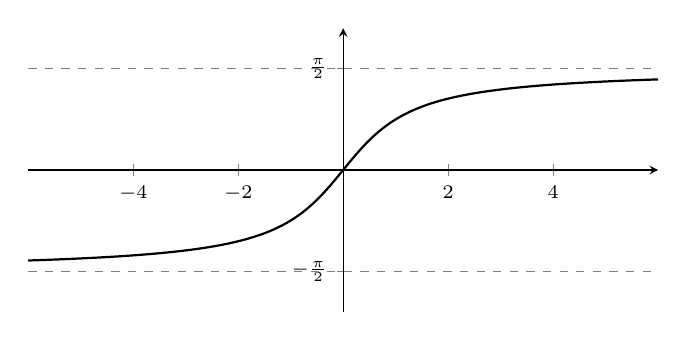
\begin{tikzpicture}
\begin{axis}[
  axis lines=middle,
  xmin=-6, xmax=6, ymin=-2.2, ymax=2.2,
  xtick={-4,-2,2,4},
  ytick={-1.5708,1.5708},
  yticklabels={$-\frac{\pi}{2}$,$\frac{\pi}{2}$},
  width=8cm, height=3.6cm, scale only axis,
  tick label style={font=\scriptsize},
]
\addplot[gray, dashed, domain=-6:6, samples=2] {1.5708};
\addplot[gray, dashed, domain=-6:6, samples=2] {-1.5708};
\addplot[thick, domain=-6:6, samples=120] {rad(atan(x))};
\end{axis}
\end{tikzpicture}
\end{center}

\begin{proposition}{逆三角関数の微分}{tb-inverse-trig-derivative}
\[
(\arcsin x)'=\frac1{\sqrt{1-x^2}},\qquad
(\arccos x)'=-\frac1{\sqrt{1-x^2}},\qquad
(\arctan x)'=\frac1{1+x^2}.
\]
\end{proposition}

\begin{proof}
公式は覚えなくても、その場で作れる。
$\theta=\arcsin x$ とおくと $\sin\theta=x$ であり、両辺を $x$ で微分すると
\[
\cos\theta\cdot\frac{\d\theta}{\d x}=1,
\qquad\text{すなわち}\qquad
\frac{\d\theta}{\d x}=\frac1{\cos\theta}.
\]
分母の $\cos\theta$ を $x$ で表せばよい。斜辺が $1$、$\theta$ の対辺が $x$ の
直角三角形を描くと、残る辺は三平方の定理から $\sqrt{1-x^2}$ である。

\begin{center}
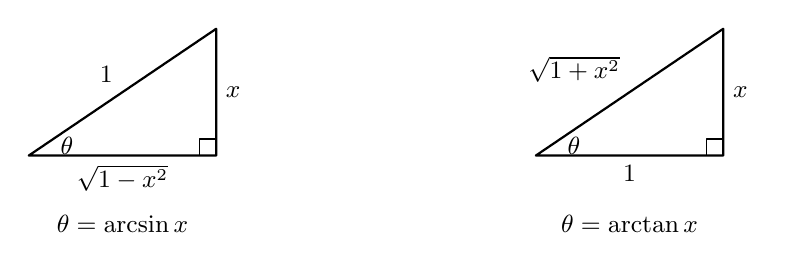
\begin{tikzpicture}[scale=1.4, line join=round]
\draw[thick] (0,0) -- (1.7,0) -- (1.7,1.15) -- cycle;
\draw (1.55,0) rectangle (1.7,0.15);
\node[below, font=\small] at (0.85,0) {$\sqrt{1-x^2}$};
\node[right, font=\small] at (1.7,0.575) {$x$};
\node[above left, font=\small] at (0.85,0.575) {$1$};
\node[right, font=\small] at (0.2,0.09) {$\theta$};
\node[font=\small] at (0.85,-0.62) {$\theta=\arcsin x$};
\begin{scope}[xshift=4.6cm]
\draw[thick] (0,0) -- (1.7,0) -- (1.7,1.15) -- cycle;
\draw (1.55,0) rectangle (1.7,0.15);
\node[below, font=\small] at (0.85,0) {$1$};
\node[right, font=\small] at (1.7,0.575) {$x$};
\node[above left, font=\small] at (0.85,0.575) {$\sqrt{1+x^2}$};
\node[right, font=\small] at (0.2,0.09) {$\theta$};
\node[font=\small] at (0.85,-0.62) {$\theta=\arctan x$};
\end{scope}
\end{tikzpicture}
\end{center}

主値では $-\pi/2\le\theta\le\pi/2$ なので $\cos\theta\ge0$ であり、
$\cos\theta=\sqrt{1-x^2}$ と符号が決まる。これで
$(\arcsin x)'=1/\sqrt{1-x^2}$ を得る。

$\arctan$ も同じ手順である。$\theta=\arctan x$ なら $\tan\theta=x$ で
\[
\sec^2\theta\cdot\frac{\d\theta}{\d x}=1,
\qquad
\frac{\d\theta}{\d x}=\frac1{\sec^2\theta}=\cos^2\theta.
\]
対辺が $x$、隣辺が $1$ の直角三角形では斜辺が $\sqrt{1+x^2}$ なので
$\cos\theta=1/\sqrt{1+x^2}$、従って $(\arctan x)'=1/(1+x^2)$ である。
\end{proof}

\begin{proposition}{$\arcsin$ と $\arccos$ の関係}{tb-arcsin-arccos}
$-1\le x\le1$ に対して
\[
\arcsin x+\arccos x=\frac\pi2.
\]
\end{proposition}

\begin{proof}
$\theta=\arcsin x$ とすると $\cos(\pi/2-\theta)=\sin\theta=x$ であり、
$-\pi/2\le\theta\le\pi/2$ から $0\le\pi/2-\theta\le\pi$ なので、
$\pi/2-\theta$ は $\arccos x$ の主値の範囲に入る。従って $\pi/2-\theta=\arccos x$ である。
\end{proof}

この式の両辺を微分すれば $(\arccos x)'=-(\arcsin x)'$ となる。
$\arccos$ の導関数が $\arcsin$ と符号だけ違うのは、
二つが $\pi/2$ を挟んで折り返しの関係にあるからである。

\section{双曲線関数}

\begin{definition}{双曲線関数}{tb-hyperbolic}
\[
\sinh x=\frac{e^x-e^{-x}}2,\qquad
\cosh x=\frac{e^x+e^{-x}}2,\qquad
\tanh x=\frac{\sinh x}{\cosh x}.
\]
\end{definition}

\begin{proposition}{双曲線関数の性質}{tb-hyperbolic-properties}
\[
\cosh^2x-\sinh^2x=1,
\qquad
(\sinh x)'=\cosh x,
\qquad
(\cosh x)'=\sinh x.
\]
また $\sinh$ の逆関数は
\[
\operatorname{arsinh}x=\log\left(x+\sqrt{x^2+1}\right)
\]
である。
\end{proposition}

\begin{example}{置換 $t=x+\sqrt{x^2+1}$}{tb-substitution-t}
$t=x+\sqrt{x^2+1}$ とおくと
\[
\left(\sqrt{x^2+1}+x\right)\left(\sqrt{x^2+1}-x\right)=(x^2+1)-x^2=1
\]
なので $t^{-1}=\sqrt{x^2+1}-x$ である。従って
\[
x=\frac{t-t^{-1}}2,\qquad
\sqrt{x^2+1}=\frac{t+t^{-1}}2,\qquad
\d x=\frac{1+t^{-2}}2\,\d t.
\]
これは $x=\sinh u$, $t=e^u$ と置いたことに他ならない。
$\sqrt{x^2+1}$ を含む積分は、この置換で有理式へ落ちる。
\end{example}

\begin{memo*}
2015年度 応用数理 専門基礎 第3問では、
$\int_0^1\d x/\sqrt{x^2+1}$ と $\int_0^1\sqrt{x^2+1}\,\d x$ を
まさにこの置換で計算する。$t$ と $t^{-1}$ を足し引きするところが要点である。
\end{memo*}

\section{よく使う不等式}

\begin{proposition}{基本不等式}{tb-basic-inequalities}
\[
\abs{\sin x}\le\abs x\quad(x\in\R),
\qquad
\abs{\sin x}\le1,
\]
\[
1+x\le e^x\quad(x\in\R),
\qquad
\log x\le x-1\quad(x>0).
\]
\end{proposition}

\begin{proposition}{相加平均・相乗平均}{tb-am-gm}
$u,v\ge0$ に対して
\[
uv\le\left(\frac{u+v}2\right)^2,
\qquad\text{すなわち}\qquad
\sqrt{uv}\le\frac{u+v}2
\]
であり、等号は $u=v$ のときに限る。
\end{proposition}

\begin{proposition}{三角不等式と Cauchy--Schwarz の不等式}{tb-triangle-cauchy}
実数・ベクトル・ノルムのいずれについても
\[
\abs{a+b}\le\abs a+\abs b,
\qquad
\bigl|\abs a-\abs b\bigr|\le\abs{a-b}
\]
が成り立つ。内積空間では
\[
\abs{\inner xy}\le\norm x\,\norm y
\]
であり、等号は $x,y$ が平行なときに限る。
\end{proposition}

「$\abs{A-B}\le C$ を示せ」という問題は、
まず $A\le B+C$ を示し、次に $A,B$ を入れ替えて $B\le A+C$ を示す、
という二段構えで書くのが定型である。
2026年度 第2期 専門基礎 第3問、2021年度 第2期 専門基礎 第3問、
年度不明の距離空間の問題はいずれもこの型である。

\section{覚えておく極限}

\begin{proposition}{標準的な極限}{tb-standard-limits}
\[
\lim_{x\to0}\frac{\sin x}x=1,
\qquad
\lim_{x\to0}\frac{1-\cos x}{x^2}=\frac12,
\qquad
\lim_{x\to0}\frac{e^x-1}x=1,
\]
\[
\lim_{x\to0}\frac{\log(1+x)}x=1,
\qquad
\lim_{n\to\infty}\left(1+\frac1n\right)^n=e,
\]
\[
\lim_{x\to\infty}\frac{\log x}{x^\alpha}=0\ (\alpha>0),
\qquad
\lim_{x\to\infty}\frac{x^\alpha}{e^x}=0,
\qquad
\lim_{x\to+0}x^\alpha\log x=0\ (\alpha>0).
\]
最後の三つは「対数は冪より遅く、冪は指数より遅い」と覚える。
\end{proposition}

これらの $x$ は、$0$ または $\infty$ へ向かう任意の式で置き換えてよい。
たとえば $h\to0$ のとき $x^2h\to0$ なので、$\lim_{x\to0}\sin x/x=1$ は
\[
\frac{\sin(x^2h)}{x^2h}\longrightarrow1
\]
の形で使える。置き換えた式が本当に $0$ または $\infty$ へ向かうことを、
使う前に確かめること。

\begin{memo*}
$\sin x/x\to1$ は、2021年度 第1期 専門基礎 第2問の偏微分の計算と、
2015年度 専門科目 第7問の優収束定理の適用で使う。
$\log x/x^\alpha\to0$ は、2015年度 第1期 専門基礎 第2問で
広義積分 $\int_1^\infty u^a\log u\,\d u$ の収束を判定するときに使う。
\end{memo*}

\chapter{一変数の微分}
\label{ch:tb-differential}

\section{出題された二つの対数微分}

$u\ne0$ では $(\log\abs u)'=u'/u$ だから
\[
\frac{\d}{\d x}\log\abs{\tan x}
=\frac{\sec^2x}{\tan x}
=\frac1{\sin x\cos x}.
\]
また変数が指数にあれば、正の範囲で指数・対数へ戻す。例えば
\[
x^{\sin x}=\exp(\sin x\log x),
\qquad
\frac{\d}{\d x}x^{\sin x}
=x^{\sin x}\left(\cos x\log x+\frac{\sin x}{x}\right).
\]

\section{最大値・最小値}

\begin{theorem}{最大値・最小値の存在}{tb-extreme-value}
コンパクト集合上の連続関数は最大値と最小値を取る。
特に $\R^n$ の有界閉集合はコンパクトである。
\end{theorem}

\begin{proposition}{無限遠で0へ収束する関数}{tb-extreme-at-infinity}
連続関数 $f:\R\to\R$ が $\abs{x}\to\infty$ で $f(x)\to0$ なら、
$f$ は最大値または最小値を持つ。
\end{proposition}

\begin{proof}
$f\equiv0$ ならよい。$f(p)\ne0$ を取り、$\varepsilon=\abs{f(p)}/2$ とする。
ある $R>\abs p$ で
\[
\abs x>R\Longrightarrow\abs{f(x)}<\varepsilon
\]
となる。$[-R,R]$ 上で取る最大・最小を $M,m$ とする。
$f(p)>0$ なら $M\ge2\varepsilon$ なので $M$ は $\R$ 全体の最大値、
$f(p)<0$ なら同様に $m$ が全体の最小値である。
\end{proof}

具体的な最大・最小は、定義域、端点、$f'=0$ となる点、無限遠での極限を調べ、
$f'$ の符号で比較する。制約に平方根があれば
$u=\sqrt x$, $v=\sqrt y$ と置いて一変数へ落とす。

\section{一様収束と誤差関数}

$f_N:I\to\R$ が $f$ に一様収束するとは
\[
\sup_{x\in I}\abs{f_N(x)-f(x)}\longrightarrow0
\]
となることをいう。

有界閉区間 $[a,b]$ 上で連続な $f_N$ が $f$ に一様収束すれば
\[
\int_a^bf_N(x)\,\d x\longrightarrow\int_a^bf(x)\,\d x.
\]
従って関数項級数の部分和が一様収束すれば項別積分できる。

2026年度第1期では、指数関数についての次の有限和と誤差だけを使う。
ある $0<\theta<1$ に対して
\[
e^t=\sum_{n=0}^{N}\frac{t^n}{n!}
+\frac{e^{\theta t}t^{N+1}}{(N+1)!}.
\]
$t=-x^2$ とし、有界閉区間上で $\abs x\le M$ と取れば
\[
\left|e^{-x^2}-\sum_{n=0}^{N}\frac{(-1)^nx^{2n}}{n!}\right|
\le\frac{(M^2)^{N+1}}{(N+1)!}\longrightarrow0.
\]
これで必要な一様収束が直接示せる。項別積分により
\[
\int_0^xe^{-t^2}\,\d t
=\sum_{n=0}^{\infty}\frac{(-1)^n}{n!(2n+1)}x^{2n+1}.
\]
$x=1$ で $N$ 次まで使ったときは、積分後の誤差も
\[
\left|\int_0^1e^{-t^2}\,\d t
-\sum_{n=0}^{N}\frac{(-1)^n}{n!(2n+1)}\right|
\le\frac1{(N+1)!(2N+3)}
\]
と評価できる。

\section{加法的関数}

\begin{theorem}{連続な Cauchy の関数方程式}{tb-cauchy-equation}
$f:\R\to\R$ が $f(x+y)=f(x)+f(y)$ を満たし、連続なら、
ある $c\in\R$ により $f(x)=cx$ と書ける。
\end{theorem}

\begin{proof}
加法性から $f(0)=0$, $f(-x)=-f(x)$ を得る。整数 $m$ と正整数 $n$ について
$f(mx)=mf(x)$, $f(x/n)=f(x)/n$ だから、有理数 $r$ では $f(rx)=rf(x)$ である。
$c=f(1)$ とし、$x$ に収束する有理数列 $r_k$ を取る。連続性から
\[
f(x)=\lim_{k\to\infty}f(r_k)=\lim_{k\to\infty}cr_k=cx.
\]
\end{proof}

\chapter{一変数の積分}
\label{ch:tb-integral}

\section{出題で使う積分操作}

変数上端には微積分学の基本定理
\[
\frac{\d}{\d x}\int_a^x f(t)\,\d t=f(x)
\]
を使う。置換積分と部分積分は
\[
\int_{\phi(\alpha)}^{\phi(\beta)}f(x)\,\d x
=\int_\alpha^\beta f(\phi(t))\phi'(t)\,\d t,
\]
\[
\int_a^bu(x)v'(x)\,\d x
=\bigl[u(x)v(x)\bigr]_a^b-\int_a^bu'(x)v(x)\,\d x
\]
である。定積分の置換では端点も変える。

2015年度第1期で必要な部分積分は、$a\ne-1$ のとき
\[
\int x^a\log x\,\d x
=x^{a+1}\left(\frac{\log x}{a+1}-\frac1{(a+1)^2}\right)+C.
\]
$a=-1$ だけは $u=\log x$ と置いて
\[
\int\frac{\log x}{x}\,\d x=\frac{(\log x)^2}{2}+C
\]
となる。$\sqrt{x^2+1}$ の置換は第\ref{ch:tb-functions}章に置いた。

\section{広義積分と比較}

非有界区間または特異点を含む積分は、端を切った積分の極限で定義する。
例えば
\[
\int_a^\infty f(x)\,\d x
=\lim_{R\to\infty}\int_a^Rf(x)\,\d x.
\]
特異点が内部にあれば左右を別々に判定する。

\[
\int_1^\infty x^a\,\d x<\infty\Longleftrightarrow a<-1,
\qquad
\int_0^1x^a\,\d x<\infty\Longleftrightarrow a>-1.
\]
$0\le f\le g$ かつ $\int g<\infty$ なら $\int f<\infty$ であり、
$\int\abs f<\infty$ なら $\int f$ は収束する。

問題の $\int_1^\infty x^a\log x\,\d x$ は $t=\log x$ により
\[
\int_0^\infty te^{(a+1)t}\,\d t
\]
へ変わるため、$a<-1$ のとき、かつそのときに限り収束する。

\section{局所化する指数核}

\begin{theorem}{近似恒等核 $ne^{-nx}$}{tb-exponential-kernel}
$f:[0,\infty)\to\R$ が有界かつ $0$ で連続なら
\[
\lim_{n\to\infty}\int_0^\infty n f(x)e^{-nx}\,\d x=f(0).
\]
\end{theorem}

\begin{proof}
$\int_0^\infty ne^{-nx}\,\d x=1$ なので、差は
\[
\int_0^\infty n\bigl(f(x)-f(0)\bigr)e^{-nx}\,\d x
\]
である。$\varepsilon>0$ に対し、$0\le x\le\delta$ で
$\abs{f(x)-f(0)}<\varepsilon$ となる $\delta$ を取る。
$M=\sup_{x\ge0}\abs{f(x)-f(0)}$ とすれば、積分を $\delta$ で分けて
\[
\left|\int_0^\infty n(f(x)-f(0))e^{-nx}\,\d x\right|
\le\varepsilon+Me^{-n\delta}\longrightarrow\varepsilon.
\]
$\varepsilon$ は任意なので結論を得る。
\end{proof}

\chapter{多変数の微分積分}
\label{ch:tb-multivariable}

\section{連続性、偏微分、\texorpdfstring{$C^1$ 級}{C1 級}}

$C^1$ 級は1階偏導関数が存在して連続、$C^\infty$ 級は全階の偏導関数が連続、という意味である。
$C^1$ 級なら連続だが、偏導関数が存在するだけでは連続とは限らない。

原点で場合分けされた関数は、次の順に処理する。
\begin{enumerate}
  \item 連続性：$x=r\cos\theta$, $y=r\sin\theta$ とし、
        $\abs{f(x,y)-f(0,0)}\le Cr^\alpha$（$\alpha>0$）へ落とす。
  \item 原点での偏微分：周囲の式を形式微分せず、軸上の差商
        \[
        f_x(0,0)=\lim_{h\to0}\frac{f(h,0)-f(0,0)}h,
        \quad
        f_y(0,0)=\lim_{h\to0}\frac{f(0,h)-f(0,0)}h
        \]
        を計算する。
  \item $C^1$ 級でないこと：周囲で偏導関数を計算し、原点へ近づける経路を一つ選んで
        不連続を示す。
\end{enumerate}
評価では $\abs{\sin u}\le\min\{\abs u,1\}$ を、原点付近と無限遠で使い分ける。

\begin{theorem}{曲線に沿う連鎖律}{tb-multivariable-chain-rule}
$f$ が $C^1$ 級で $x(t),y(t)$ が微分可能なら
\[
\frac{\d}{\d t}f(x(t),y(t))
=f_x(x(t),y(t))x'(t)+f_y(x(t),y(t))y'(t).
\]
\end{theorem}

\begin{proposition}{原点で消える滑らかな関数の分解}{tb-smooth-factorization}
$f\in C^\infty(\R^2)$, $f(0,0)=0$ なら
\[
f(x,y)=xg(x,y)+yh(x,y)
\]
となる $g,h\in C^\infty(\R^2)$ が存在する。さらに
\[
f(x,y)=xG(x,y)+yH(y)
\]
という形にもできる。
\end{proposition}

\begin{proof}
$F(t)=f(tx,ty)$ とおく。基本定理と連鎖律から
\[
f(x,y)=\int_0^1F'(t)\,\d t
=x\int_0^1f_x(tx,ty)\,\d t
+y\int_0^1f_y(tx,ty)\,\d t.
\]
これが最初の表示である。二つ目は
\[
f(x,y)=\bigl(f(x,y)-f(0,y)\bigr)+f(0,y)
=x\int_0^1 f_x(tx,y)\,\d t
+y\int_0^1f_y(0,ty)\,\d t
\]
とすればよい。被積分関数が滑らかなので、得られた関数も滑らかである。
\end{proof}

\section{積分記号下の微分}

積分区間が動くか、中身だけが動くかを最初に分ける。

\begin{theorem}{Leibniz 則}{tb-leibniz-rule}
$f,f_x$ が必要な長方形上で連続なら
\[
\frac{\d}{\d x}\int_c^d f(x,y)\,\d y
=\int_c^d f_x(x,y)\,\d y.
\]
さらに $\phi,\psi$ が $C^1$ 級なら
\[
\frac{\d}{\d x}\int_{\phi(x)}^{\psi(x)}f(x,y)\,\d y
=f(x,\psi(x))\psi'(x)-f(x,\phi(x))\phi'(x)
+\int_{\phi(x)}^{\psi(x)}f_x(x,y)\,\d y.
\]
\end{theorem}

右辺は順に「上端」「下端」「中身」の変化である。
証明は $Q(x,v)=\int_c^v f(x,y)\,\d y$ と置き、
$Q(x,\psi(x))-Q(x,\phi(x))$ に二変数の連鎖律を使う。

例えば
\[
f(x)=\int_a^x\d s\int_a^s u(s,t)\,\d t
\]
では、外側の基本定理だけで
$f'(x)=\int_a^xu(x,t)\,\d t$ となる。

\begin{theorem}{パラメータ積分の微分}{tb-differentiate-integral}
$t$ がコンパクト区間を動き、$f(t,x)$ と $f_t(t,x)$ が連続で、
$\abs{f_t(t,x)}\le g(x)$ となる可積分関数 $g$ があれば
\[
\frac{\d}{\d t}\int f(t,x)\,\d x=\int f_t(t,x)\,\d x.
\]
広義積分では、交換を正当化する優関数 $g$ を答案に書く。
\end{theorem}

答案では「形式微分したら簡単になった」で終えない。
$t$ の近傍を固定し、そこで共通に使える可積分な $g(x)$ を一つ書く。

\begin{example}{$(x^t-1)/\log x$}{tb-log-quotient-parameter}
$0<x<1$, $t\ge0$ では
\[
\frac{x^t-1}{\log x}=\int_0^t x^s\,\d s.
\]
この表示から $0\le (x^t-1)/\log x\le t$、$x\to1$ での極限が $t$ と分かる。
さらに $t$ で微分すれば $x^t$ なので
\[
\frac{\d}{\d t}\int_0^1\frac{x^t-1}{\log x}\,\d x
=\int_0^1x^t\,\d x=\frac1{t+1}.
\]
積分表示は端点の特異性、評価、微分を同時に処理する。
\end{example}

\section{重積分と変数変換}

被積分関数より先に領域を見る。直交座標のまま上下端が一行で書けるなら累次積分、
円・和・比が境界に現れるなら変数変換を選ぶ。

\begin{theorem}{Fubini--Tonelli}{tb-fubini-tonelli}
$f\ge0$ なら Tonelli の定理により累次積分の順序を交換できる。
符号を持つ $f$ では $\iint\abs f<\infty$ なら Fubini の定理により交換できる。
有界閉領域上の連続関数では後者の条件が自動的に成り立つ。
\end{theorem}

累次積分へ直す前に領域を図示し、例えば
\[
D=\{(x,y)\mid a\le x\le b,\ \phi(x)\le y\le\psi(x)\}
\]
の形へ書く。境界の上下関係が変わる点で積分区間を分ける。

\begin{theorem}{二変数の変数変換}{tb-change-of-variables}
$\Phi:(u,v)\mapsto(x,y)$ が領域間の $C^1$ 級全単射で、内部で Jacobian が消えないなら
\[
\iint_D f(x,y)\,\d x\d y
=\iint_{\Phi^{-1}(D)}f(\Phi(u,v))
\left|\frac{\partial(x,y)}{\partial(u,v)}\right|\d u\d v.
\]
掛けるのは
\[
\left|\frac{\partial(x,y)}{\partial(u,v)}\right|
=\left|\det
\begin{pmatrix}x_u&x_v\\y_u&y_v\end{pmatrix}\right|
\]
であり、絶対値を忘れない。
\end{theorem}

変数変換は次の順に行う。
\begin{enumerate}
  \item 逆変換を求める。
  \item 領域の全ての不等式を新変数へ移し、新領域を確定する。
  \item Jacobian の絶対値を計算する。
  \item 被積分関数と面積要素を両方置き換える。
\end{enumerate}

\begin{proposition}{頻出する変換}{tb-standard-transformations}
\[
\begin{array}{c|c|c}
\text{目的}&(x,y)&\left|\partial(x,y)/\partial(u,v)\right|\\ \hline
\text{極座標}&(r\cos\theta,r\sin\theta)&r\\
x+y,\ x-y&( (u+v)/2,(u-v)/2)&1/2\\
\text{合計と割合}&(st,s(1-t))&s\\
\text{平方した極座標}&((r\cos\theta)^2,(r\sin\theta)^2)&4r^3\sin\theta\cos\theta
\end{array}
\]
最後の二行では通常 $s>0$, $0<t<1$ および $r>0$, $0<\theta<\pi/2$ を使う。
\end{proposition}

極座標で $0\le x\le1$ は $0\le r\cos\theta\le1$ となる。
$1\le r\le2$ と同時に課されるなら $r\le\min\{2,\sec\theta\}$ であり、
$\sec\theta=2$ となる $\theta=\pi/3$ で領域を分ける。

\begin{proposition}{対称性}{tb-symmetry-vanishing}
領域 $D$ が変換 $T$ で不変、Jacobian の絶対値が1で、
$f(Tx)=-f(x)$ なら $\int_Df=0$ である。
特に原点対称な領域上では、奇関数の積分は0になる。
\end{proposition}

\begin{proposition}{Gaussian 積分}{tb-gaussian-integral}
\[
\int_0^\infty e^{-x^2}\,\d x=\frac{\sqrt\pi}{2}.
\]
\end{proposition}

\begin{proof}
$I_R=\int_0^Re^{-x^2}\,\d x$ とし、$S_R=[0,R]^2$ とおくと Fubini の定理により
\[
I_R^2=\iint_{S_R}e^{-(x^2+y^2)}\,\d x\d y.
\]
第1象限の半径 $a$ の四分円を $D_a$ とすれば
$D_R\subset S_R\subset D_{\sqrt2R}$ である。極座標により
\[
\iint_{D_a}e^{-(x^2+y^2)}\,\d x\d y
=\int_0^{\pi/2}\!\int_0^a e^{-r^2}r\,\d r\d\theta
=\frac\pi4(1-e^{-a^2}).
\]
両側から挟んで $R\to\infty$ とすると $I_R^2\to\pi/4$。
$I_R\ge0$ なので結論を得る。
\end{proof}

\section{Gamma・Beta 関数}

\begin{definition}{Gamma・Beta 関数}{tb-gamma-beta}
$p,q>0$ に対し
\[
\Gamma(p)=\int_0^\infty x^{p-1}e^{-x}\,\d x,
\qquad
B(p,q)=\int_0^1t^{p-1}(1-t)^{q-1}\,\d t.
\]
\end{definition}

\begin{theorem}{Beta--Gamma 関係式}{tb-beta-gamma-relation}
\[
B(p,q)=\frac{\Gamma(p)\Gamma(q)}{\Gamma(p+q)}.
\]
\end{theorem}

\begin{proof}
積を第1象限の積分
\[
\Gamma(p)\Gamma(q)=\iint x^{p-1}y^{q-1}e^{-(x+y)}\,\d x\d y
\]
にする。$x=st$, $y=s(1-t)$ を使えば
\[
\int_0^\infty s^{p+q-1}e^{-s}\,\d s
\int_0^1t^{p-1}(1-t)^{q-1}\,\d t
=\Gamma(p+q)B(p,q).
\]
別解では $x=(r\cos\theta)^2$, $y=(r\sin\theta)^2$ とし、
Jacobian $4r^3\sin\theta\cos\theta$ を掛ける。$r$ と $\theta$ の積分に分離した後、
$s=r^2$, $t=\cos^2\theta$ と置けば同じ二因子を得る。
\end{proof}

\section{円板を広げる極限}

2021年度第1期では、非負関数を円板 $B(R)$ 上で積分する。
$B(R)$ は $R$ とともに増大するので、単調収束定理から
\[
\lim_{R\to\infty}\iint_{B(R)}F
=\iint_{\R^2}F
\]
となる。右辺が有限であることは原点と無限遠を分けて評価する。
問題の関数では、極座標で
\[
\abs f\le r\quad(0<r\le1),\qquad
\abs f\le r^{-2}\quad(r\ge1)
\]
なら、$p>1$ に対し
\[
\iint\abs f^p
\le2\pi\left(\int_0^1r^{p+1}\,\d r+\int_1^\infty r^{1-2p}\,\d r\right)<\infty.
\]
原点と無限遠で別の評価を使う典型である。

\chapter{線形代数I：空間・写像・行列}
\label{ch:tb-linear-one}

\section{部分空間、基底、次元}

\begin{definition}{部分空間}{tb-subspace}
実または複素ベクトル空間 $V$ の空でない部分集合 $W$ が\textbf{部分空間}であるとは
\[
u,v\in W,\ \alpha,\beta\in\mathbb F
\Longrightarrow \alpha u+\beta v\in W
\]
を満たすことをいう。$0\in W$ と加法・スカラー倍についての閉性を別々に確認してもよい。
\end{definition}

\begin{proposition}{共通部分と合併}{tb-subspace-intersection-union}
部分空間 $U,W\subset V$ に対し $U\cap W$ は部分空間である。
$U\cup W$ が部分空間となるための必要十分条件は
$U\subset W$ または $W\subset U$ である。
\end{proposition}

\begin{proof}
共通部分では線形結合が $U,W$ の両方に残る。
合併について、どちらの包含も成り立たないなら
$u\in U\setminus W$, $w\in W\setminus U$ を取れる。
$u+w\in U\cup W$ と仮定すると、$u+w\in U$ なら $w\in U$、
$u+w\in W$ なら $u\in W$ となり、いずれも矛盾する。
\end{proof}

\begin{definition}{生成・一次独立・基底}{tb-basis}
$v_1,\ldots,v_m$ の一次結合全体を
\[
\operatorname{span}\{v_1,\ldots,v_m\}
=\left\{\sum_{i=1}^m a_iv_i\ \middle|\ a_i\in\mathbb F\right\}
\]
と書く。$\sum a_iv_i=0\Rightarrow a_1=\cdots=a_m=0$ のとき一次独立という。
一次独立で $V$ を生成する組を基底といい、有限次元空間の基底の本数を $\dim V$ とする。
\end{definition}

基底であることは「一次独立」と「生成」の二項目を示す。
行列の列ベクトルなら、pivot 列が像の基底、自由変数の本数が核の次元を与える。

\begin{definition}{和と直和}{tb-direct-sum}
\[
U+W=\{u+w\mid u\in U,w\in W\}.
\]
$U\cap W=\{0\}$ のとき $U+W$ を $U\oplus W$ と書く。
この条件は表示 $v=u+w$ の一意性と同値である。
\end{definition}

\begin{theorem}{次元公式}{tb-dimension-formula}
有限次元部分空間 $U,W$ に対し
\[
\dim(U+W)=\dim U+\dim W-\dim(U\cap W).
\]
特に直和なら $\dim(U\oplus W)=\dim U+\dim W$ である。
\end{theorem}

\section{線形写像、核、像}

\begin{definition}{線形写像と核・像}{tb-linear-map}
$f:U\to V$ が
$f(\alpha x+\beta y)=\alpha f(x)+\beta f(y)$ を満たすとき線形写像という。
\[
\ker f=\{x\in U\mid f(x)=0\},\qquad
\operatorname{Im}f=\{f(x)\mid x\in U\}.
\]
どちらも部分空間である。
\end{definition}

\begin{theorem}{単射判定と次元定理}{tb-rank-nullity}
\[
f\text{ が単射}\Longleftrightarrow\ker f=\{0\}.
\]
$U$ が有限次元なら
\[
\dim U=\dim\ker f+\dim\operatorname{Im}f.
\]
同じ有限次元空間の間の線形写像では、単射、全射、全単射が同値である。
\end{theorem}

行列 $A$ が表す写像では、$A$ の pivot 列が $\operatorname{Im}A$ の基底を与え、
$Ax=0$ の一般解から $\ker A$ の基底を得る。
二つの像の共通部分は
\[
Au=Bv\Longleftrightarrow
\begin{pmatrix}A&-B\end{pmatrix}
\binom uv=0
\]
を解き、得られた $Au$ から一次独立なものを選べばよい。

\begin{proposition}{同型写像は基底を基底へ送る}{tb-isomorphism-basis}
$f:V\to V$ が線形同型で $v_1,\ldots,v_n$ が基底なら
$f(v_1),\ldots,f(v_n)$ も基底である。
\end{proposition}

\begin{proof}
$\sum a_if(v_i)=0$ なら線形性により $f(\sum a_iv_i)=0$ である。
単射性から $\sum a_iv_i=0$、基底の一次独立性から全ての $a_i=0$ となる。
本数が $\dim V$ に等しいため、これは基底である。
\end{proof}

\begin{proposition}{像が直和である二写像}{tb-two-map-direct-sum}
$f,g:\mathbb F^n\to\mathbb F^n$ が
$\mathbb F^n=\operatorname{Im}f\oplus\operatorname{Im}g$ を満たすなら
\[
\ker(f+g)=\ker f\cap\ker g.
\]
さらに $\mathbb F^n=\ker f+\ker g$ なら $f+g$ は全単射である。
\end{proposition}

\begin{proof}
$(f+g)x=0$ なら $f(x)=-g(x)$ は二つの像の共通部分に属する。
直和なので両方0となる。逆包含は直ちに従う。
さらに次元定理と像の直和から
\[
\dim\ker f+\dim\ker g
=2n-\dim\operatorname{Im}f-\dim\operatorname{Im}g=n.
\]
一方、核の和が全空間なら次元公式により
\[
n=\dim(\ker f+\ker g)
=n-\dim(\ker f\cap\ker g).
\]
従って $\ker(f+g)=\ker f\cap\ker g=\{0\}$ であり、$f+g$ は全単射である。
\end{proof}

\section{行基本変形と連立方程式}

行基本変形は
\begin{enumerate}
  \item 二行を交換する、
  \item 一行を0でない定数倍する、
  \item 一行に別の行の定数倍を加える
\end{enumerate}
の三つであり、連立方程式の解集合を変えない。

拡大係数行列を階段形にし、
\[
\operatorname{rank}A=\operatorname{rank}(A\mid b)
\]
なら $Ax=b$ は解を持つ。pivot のない列に自由変数を置き、全ての解を書く。
斉次方程式 $Ax=0$ の解空間は $\ker A$ であり
\[
\dim\ker A=n-\operatorname{rank}A.
\]
正則行列の逆行列は Gauss--Jordan 法
$(A\mid I)\longrightarrow(I\mid A^{-1})$ で同時に求められる。

$A$ が正則なら、行列方程式は掛ける側に注意して
\[
XA=B\Longrightarrow X=BA^{-1},\qquad
AY=C\Longrightarrow Y=A^{-1}C
\]
と解く。

\section{三角行列と二段階解法}

\begin{proposition}{前進代入・後退代入}{tb-triangular-systems}
対角成分が全て0でない下三角行列 $L$ に対する $Ly=b$ は、
第1式から順に $y_1,y_2,\ldots$ を決める\textbf{前進代入}で一意に解ける。
上三角行列 $U$ に対する $Ux=y$ は、最終式から逆順に決める\textbf{後退代入}で解ける。
\end{proposition}

$A=LU$ と分解できれば
\[
Ax=b\Longleftrightarrow L(Ux)=b
\]
なので、まず $Ly=b$、次に $Ux=y$ を解けばよい。また
\[
\det A=\det L\det U
=\left(\prod_i l_{ii}\right)\left(\prod_i u_{ii}\right).
\]
特に $L$ の対角成分が全て1なら $\det A$ は $U$ の対角成分の積である。

$L$ と $A$ から $A=LU$ の $U$ を求めるときも前進代入と同じ順序を使う。
$L$ の対角成分が1なら、行ベクトルを $A_i,U_i$ と書いて
\[
U_i=A_i-\sum_{k<i}l_{ik}U_k
\]
と上の行から順に決定できる。

\section{行列式と正則性}

\begin{proposition}{行列式の計算規則}{tb-determinant-properties}
\[
\det(AB)=\det A\det B,\quad
\det A^{\mathsf T}=\det A,\quad
\det(cA)=c^n\det A.
\]
行交換で符号が反転し、一行の $c$ 倍で行列式も $c$ 倍、
一行に他の行の倍を加えても行列式は変わらない。
三角行列の行列式は対角成分の積である。
\end{proposition}

\begin{theorem}{正則性の同値条件}{tb-invertibility}
$n$ 次正方行列 $A$ について次は同値である。
\[
A\text{ は正則},\quad \det A\ne0,\quad \operatorname{rank}A=n,
\quad\ker A=\{0\},\quad Ax=b\text{ は任意の }b\text{ に一意解を持つ}.
\]
\end{theorem}

行列式は存在・非存在の証明にも使う。実行列で $A^2=-I_n$ なら
\[
(\det A)^2=\det(-I_n)=(-1)^n.
\]
左辺は非負なので $n$ は偶数である。$n=2$ では
$\begin{pmatrix}0&-1\\1&0\end{pmatrix}$ が例になる。
一方、任意の実ベクトル $x$ に対し
$x^{\mathsf T}A^{\mathsf T}Ax=\norm{Ax}^2\ge0$ なので
$A^{\mathsf T}A=-I_n$ は不可能である。

\section{行列多項式から逆行列を作る}

\begin{proposition}{逆行列を式から読む}{tb-polynomial-inverse}
$A^2+A-2I=O$ なら
\[
A(A+I)=2I,\qquad A^{-1}=\frac12(A+I).
\]
一般に $Aq(A)=cI$（$c\ne0$）まで変形できれば $A^{-1}=q(A)/c$ である。
また $N^m=O$ なら
\[
(I-N)^{-1}=I+N+\cdots+N^{m-1},\qquad
(I+N)^{-1}=I-N+\cdots+(-N)^{m-1}.
\]
\end{proposition}

積を実際に掛けて $I-N^m=I$ または $I-(-N)^m=I$ になることを示せば、
正則性と逆行列を同時に証明できる。

\chapter{線形代数II：固有値・内積・標準形}
\label{ch:tb-linear-two}

\section{固有値と対角化}

\begin{definition}{固有値・固有空間}{tb-eigenvalue}
$Av=\lambda v$ を満たす $v\ne0$ が存在するとき、$\lambda$ を $A$ の固有値、
$v$ を固有ベクトルという。
\[
E_\lambda=\ker(A-\lambda I)
\]
を固有空間という。固有多項式を
$\chi_A(t)=\det(tI-A)$ とする。
\end{definition}

固有値と固有空間は
\begin{enumerate}
  \item $\chi_A(t)$ を因数分解して固有値を得る。
  \item 各 $\lambda$ で $(A-\lambda I)v=0$ を行基本変形し、基底を求める。
\end{enumerate}
の順で計算する。$\det A$ は固有値の積、$\tr A$ は固有値の和である
（重複度を込める）。

\begin{definition}{対角化}{tb-diagonalization}
正則行列 $P=(v_1\ \cdots\ v_n)$ に対し
\[
P^{-1}AP=\diag(\lambda_1,\ldots,\lambda_n)
\]
となることを対角化という。これは $v_1,\ldots,v_n$ が固有ベクトルからなる基底であることと同値である。
\end{definition}

固有値 $\lambda$ の固有多項式での重複度を代数的重複度 $m_a(\lambda)$、
$\dim E_\lambda$ を幾何的重複度 $m_g(\lambda)$ といい
\[
1\le m_g(\lambda)\le m_a(\lambda).
\]
固有多項式が基礎体上で一次式に分解するとき、
全ての固有値で両者が等しいことと対角化可能であることは同値である。
相異なる固有値の固有ベクトルは一次独立なので、固有値が $n$ 個あれば自動的に対角化できる。

\begin{proposition}{行列が満たす多項式の使い方}{tb-matrix-polynomial}
$p(A)=O$ なら、$A$ の固有値 $\lambda$ は全て $p(\lambda)=0$ を満たす。
さらに
\[
p(t)=\prod_{i=1}^r(t-\lambda_i)\qquad(\lambda_i\ne\lambda_j\ (i\ne j))
\]
と相異なる一次式に分解できれば、$A$ は対角化可能である。このとき固有値 $\lambda_i$ の成分は
\[
P_i x=\prod_{j\ne i}\frac{A-\lambda_jI}{\lambda_i-\lambda_j}\,x
\]
で取り出せ、$x=\sum_iP_ix$、$P_ix\in E_{\lambda_i}$ となる。
\end{proposition}

$Av=\lambda v$ なら $p(A)v=p(\lambda)v$ なので前半が従う。
後半は Lagrange 補間の恒等式 $\sum_iP_i=I$ と
$(A-\lambda_iI)P_i=O$ を用いればよい。

対角化できれば
\[
A^k=PD^kP^{-1},\qquad
D^k=\diag(\lambda_1^k,\ldots,\lambda_n^k).
\]
行列で表された漸化式 $X_n=AX_{n-1}$ も $X_n=A^{n-n_0}X_{n_0}$ として同じ方法で解く。

\section{冪零行列と Jordan 標準形}

\begin{definition}{冪零と Jordan ブロック}{tb-jordan}
$N^m=O$ となる正整数 $m$ が存在するとき $N$ を冪零という。
\[
J_k(\lambda)=
\begin{pmatrix}
\lambda&1&&0\\
&\lambda&\ddots&\\
&&\ddots&1\\
0&&&\lambda
\end{pmatrix}
\]
を Jordan ブロックといい、これらを対角に並べた行列を Jordan 標準形という。
\end{definition}

冪零行列の固有値は0だけである。実際 $Nv=\lambda v$ なら
$0=N^mv=\lambda^mv$ なので $\lambda=0$ である。
したがって全ての $k\ge1$ で $\tr N^k=0$ となる。

\begin{proposition}{Jordan ブロックの読み方}{tb-jordan-nullities}
固有値 $\lambda$ について $N=A-\lambda I$ とする。
\begin{itemize}
  \item ブロックの個数は $\dim\ker N$。
  \item 大きさ $j$ 以上のブロックの個数は
        $\dim\ker N^j-\dim\ker N^{j-1}$。
  \item 最大ブロックの大きさは $N^j$ が一般化固有空間上で0になる最小の $j$。
\end{itemize}
\end{proposition}

3次で固有値が一つなら、$\dim\ker N=3,2,1$ に応じてブロック型は
$1+1+1$, $2+1$, または $3$ である。
パラメータを含む問題では、固有値が衝突する値を先に分けて核の次元を調べる。

\section{不変部分空間と上三角化}

\begin{definition}{不変部分空間}{tb-invariant-subspace}
$W\subset V$ が $A$ 不変であるとは $AW\subset W$ をいう。
1次元不変部分空間は固有ベクトル $v$ が張る直線 $\operatorname{span}\{v\}$ に限る。
\end{definition}

$V=\R^3$ の2次元部分空間は $W=\ker \ell$（$\ell\ne0$ は行ベクトル）と書ける。
このとき
\[
AW\subset W
\Longleftrightarrow \ell A=\lambda\ell\text{ となる }\lambda\text{ が存在する}.
\]
したがって2次元不変部分空間は $A^{\mathsf T}$ の固有ベクトル $u$ を求め、
$W=\{x\mid u^{\mathsf T}x=0\}$ とすれば分類できる。

\begin{theorem}{不変旗と上三角化}{tb-invariant-flag}
基底 $v_1,\ldots,v_n$ と
$W_j=\operatorname{span}\{v_1,\ldots,v_j\}$ が全て $AW_j\subset W_j$ を満たすとする。
$P=(v_1\ \cdots\ v_n)$ とおけば $P^{-1}AP$ は上三角行列である。
\end{theorem}

\begin{proof}
$Av_j\in W_j$ なので
$Av_j=\sum_{i=1}^j t_{ij}v_i$ と書ける。
これは $AP=PT$ の第 $j$ 列であり、$i>j$ の成分 $t_{ij}$ が0、すなわち $T$ が上三角であることを意味する。
\end{proof}

\section{内積、直交行列、ユニタリ行列}

実内積を $\inner{x}{y}=x^{\mathsf T}y$、複素内積を $\inner{x}{y}=x^*y$、
$\norm{x}=\sqrt{\inner{x}{x}}$ とする。
実内積はノルムから
\[
\inner{x}{y}=\frac12\left(\norm{x+y}^2-\norm{x}^2-\norm{y}^2\right)
\]
と復元できる。

一次独立な $v_1,\ldots,v_m$ は Gram--Schmidt 法
\[
u_1=v_1,\qquad
u_k=v_k-\sum_{j=1}^{k-1}
\frac{\inner{u_j}{v_k}}{\inner{u_j}{u_j}}u_j,\qquad
e_k=\frac{u_k}{\norm{u_k}}
\]
で正規直交系 $e_1,\ldots,e_m$ にできる。
固有空間の中でこの操作を行っても、得られるベクトルは同じ固有空間に残る。

\begin{definition}{直交行列・ユニタリ行列}{tb-orthogonal-unitary}
実行列 $Q$ が $Q^{\mathsf T}Q=I$ を満たすとき直交行列、
複素行列 $U$ が $U^*U=I$ を満たすときユニタリ行列という。
列ベクトルが正規直交基底であることと同値であり
\[
Q^{-1}=Q^{\mathsf T},\qquad U^{-1}=U^*.
\]
\end{definition}

\begin{proposition}{長さ・内積・直交性の同値}{tb-isometry-equivalence}
実正方行列 $Q$ について次は同値である。
\[
Q^{\mathsf T}Q=I,\qquad
\norm{Qx}=\norm x\ (\forall x),\qquad
\inner{Qx}{Qy}=\inner{x}{y}\ (\forall x,y).
\]
\end{proposition}

\begin{proof}
最初から最後は $\inner{Qx}{Qy}=x^{\mathsf T}Q^{\mathsf T}Qy$ で従う。
長さの保存から内積の保存は上の偏極公式を使う。
内積の保存からは
$x^{\mathsf T}(Q^{\mathsf T}Q-I)y=0$ が全ての $x,y$ で成り立つため $Q^{\mathsf T}Q=I$ である。
\end{proof}

3次直交行列の二列が分かっているとき、残る単位列ベクトルはその外積の $\pm$ である。
最後に行列式の符号や与えられた成分でどちらかを選ぶ。
また $(Q^{\mathsf T})^k=Q^{-k}$ なので、直交行列の複雑な積は指数法則へ直す。

\section{対称・交代・エルミート行列}

\begin{definition}{三つの行列}{tb-symmetric-hermitian}
\[
A^{\mathsf T}=A:\text{実対称},\qquad
A^{\mathsf T}=-A:\text{実交代},\qquad
A^*=A:\text{エルミート}.
\]
\end{definition}

\begin{theorem}{スペクトル定理}{tb-spectral-theorem}
実対称行列は直交行列で、エルミート行列はユニタリ行列で対角化できる。
固有値は全て実数であり、相異なる固有値の固有空間は互いに直交する。
\end{theorem}

ユニタリ対角化では、各固有空間の基底を求め、重複固有値の固有空間内で
Gram--Schmidt 法を使い、得られた正規直交固有ベクトルを列に並べる。

逆に、実行列が直交行列 $Q$ と実対角行列 $D$ により
$A=QDQ^{\mathsf T}$ と書けるなら
$A^{\mathsf T}=QD^{\mathsf T}Q^{\mathsf T}=A$ なので $A$ は対称行列である。

エルミート行列 $A$ で $Av=\lambda v$ とすれば
\[
\lambda\norm v^2=v^*Av=(v^*Av)^*=\overline\lambda\norm v^2
\]
なので $\lambda\in\R$ である。
相異なる固有値 $\lambda,\mu$ の固有ベクトル $v,w$ について
$\lambda\inner{v}{w}=\inner{Av}{w}=\inner{v}{Aw}=\mu\inner{v}{w}$ だから直交する。

非零の実交代行列は実数上で対角化できない。実固有値 $\lambda$ と実固有ベクトル $v$ に対し
\[
\lambda\norm v^2=v^{\mathsf T}Av
=(v^{\mathsf T}Av)^{\mathsf T}=v^{\mathsf T}A^{\mathsf T}v=-v^{\mathsf T}Av
\]
より $\lambda=0$ である。実対角化できるなら全固有値が0なので行列自体が0となり、仮定に反する。

\section{二次形式と行列空間}

\begin{theorem}{Rayleigh 商}{tb-rayleigh}
実対称行列 $A$ の最小・最大固有値を $\lambda_{\min},\lambda_{\max}$ とすると
\[
\lambda_{\min}\le\frac{x^{\mathsf T}Ax}{x^{\mathsf T}x}\le\lambda_{\max}\qquad(x\ne0).
\]
単位球面上の $x^{\mathsf T}Ax$ の最大値・最小値は両端の固有値であり、
等号は対応する固有空間上で成立する。
\end{theorem}

$n$ 次実対称行列全体の次元は、対角成分 $n$ と上三角部分 $n(n-1)/2$ を合わせて
$n(n+1)/2$ である。実交代行列全体の次元は $n(n-1)/2$ である。

\begin{definition}{Frobenius 内積}{tb-frobenius}
同じサイズの実行列に
\[
\inner{A}{B}_{F}=\tr(A^{\mathsf T}B)
\]
と定める。特に列ベクトル $x,y$ に対し
\[
\inner{xx^{\mathsf T}}{yy^{\mathsf T}}_F=(x^{\mathsf T}y)^2.
\]
\end{definition}

$\sum_i a_ix_ix_i^{\mathsf T}=O$ の両辺と $x_jx_j^{\mathsf T}$ の Frobenius 内積を取ると
\[
\sum_i a_i(x_i^{\mathsf T}x_j)^2=0.
\]
係数行列が正則と分かれば全ての $a_i=0$、従って外積行列は一次独立である。
特に $\norm{x_i}=1$, $\abs{\inner{x_i}{x_j}}=r$（$i\ne j$, $0\le r<1$）なら、
$S=\sum_i a_i$ とおくことで各式は
\[
(1-r^2)a_j+r^2S=0
\]
となる。全ての $a_j$ は等しく、元の式から
$[1+(n-1)r^2]a_j=0$、従って全て0である。
3次対称行列空間の次元は6なので、そのような行列は高々6個しか存在できない。

\chapter{距離空間と位相}
\label{ch:tb-topology}

位相では定義そのものが答案の初手になるため、ここだけは開・閉・コンパクト・連結を正確に言えるようにする。
証明全文を暗記する必要はなく、「開被覆を逆像へ戻す」「二点の間で切る」などの操作を再現する。

\section{開集合・閉集合・閉包}

\begin{definition}{距離空間と開球}{tb-metric-space}
集合 $X$ 上の距離 $d$ は
\[
d(x,y)\ge0,\quad d(x,y)=0\Longleftrightarrow x=y,\quad
d(x,y)=d(y,x),\quad d(x,z)\le d(x,y)+d(y,z)
\]
を満たす。$B(x;r)=\{y\in X\mid d(x,y)<r\}$ を開球という。
\end{definition}

\begin{definition}{開集合・閉集合・閉包}{tb-open-closed-closure}
$U\subset X$ が開集合であるとは、各 $x\in U$ に対し
$B(x;r)\subset U$ となる $r>0$ が存在することをいう。
$F\subset X$ が閉集合であるとは $X\setminus F$ が開集合であることをいう。
$A$ を含む最小の閉集合を閉包 $\overline A$ といい、
$x\in\overline A$ を $A$ の触点という。
\end{definition}

距離空間では
\[
x\in\overline A
\Longleftrightarrow \forall r>0,\ B(x;r)\cap A\ne\varnothing
\Longleftrightarrow A\text{ の点列 }a_n\to x\text{ が存在する}.
\]
$\overline A=X$ のとき $A$ は $X$ で稠密という。

閉包を求める問題では、まず集合内の典型的な点列の極限を探す。
閉集合を示すときは、補集合が開であることと、収束列の極限を含むことの短い方を選ぶ。

\begin{proposition}{閉包の計算法則}{tb-closure-laws}
\[
A\subset\overline A,\quad
\overline{\overline A}=\overline A,\quad
A\subset B\Rightarrow\overline A\subset\overline B,\quad
\overline{A\cup B}=\overline A\cup\overline B.
\]
\end{proposition}

最後の式は、右辺が $A\cup B$ を含む閉集合なので一方の包含を得る。
逆包含は $A,B\subset A\cup B$ の単調性から得る。

\begin{definition}{相対位相}{tb-subspace-topology}
$Y\subset X$ に対し、$Y$ の開集合を $Y\cap U$（$U$ は $X$ の開集合）と定める。
閉集合も $Y\cap F$（$F$ は $X$ の閉集合）の形である。
したがって $[1,2]\cap\Q$ は $\Q$ の中では閉集合である。
\end{definition}

\begin{definition}{位相空間と Hausdorff 性}{tb-topological-space}
集合 $X$ の部分集合族 $\mathcal T$ が
\[
\varnothing,X\in\mathcal T,\qquad
\mathcal T\text{ の任意個の元の合併が }\mathcal T\text{ に属する},
\]
\[
\mathcal T\text{ の有限個の元の共通部分が }\mathcal T\text{ に属する}
\]
を満たすとき $(X,\mathcal T)$ を位相空間という。$\mathcal T$ の元を開集合、補集合を閉集合と呼ぶ。
異なる二点が互いに交わらない開近傍で分離できるとき Hausdorff 空間という。
\end{definition}

\begin{definition}{点列の収束}{tb-topological-sequence}
位相空間 $X$ の点列 $a_n$ が $a\in X$ に収束するとは、
$a$ の任意の開近傍 $U$ に対し、ある $N$ が存在して
\[
n\ge N\Longrightarrow a_n\in U
\]
となることをいう。
\end{definition}

\begin{proposition}{Hausdorff 空間では極限が一意}{tb-hausdorff-limit}
Hausdorff 空間の点列が極限を持つなら、その極限は一つだけである。
\end{proposition}

\begin{proof}
$a_n\to a,b$ かつ $a\ne b$ と仮定する。Hausdorff 性により
$a\in U$, $b\in V$, $U\cap V=\varnothing$ となる開近傍を取れる。
十分大きい $n$ では $a_n\in U$ かつ $a_n\in V$ となり矛盾する。
\end{proof}

\begin{proposition}{補有限位相}{tb-cofinite-topology}
無限集合 $X$ に
\[
\mathcal T=\{\varnothing\}\cup
\{U\subset X\mid X\setminus U\text{ は有限集合}\}
\]
を入れると位相空間になり、コンパクトかつ連結である。
\end{proposition}

任意個の合併の補集合は有限集合の一つに含まれ、有限個の共通部分の補集合は
有限集合の有限合併なので、位相の公理を満たす。
開被覆から非空な一つ $U_0$ を選べば $X\setminus U_0$ は有限であり、
残る各点を覆う開集合を一つずつ足せば有限部分被覆になる。
また二つの非空開集合の共通部分は補有限、従って空でない。
よって二つの非空開集合による分離は存在しない。

\section{連続写像}

\begin{definition}{連続性}{tb-metric-continuity}
距離空間の写像 $f:X\to Y$ が $x\in X$ で連続であるとは
\[
\forall\varepsilon>0\ \exists\delta>0\ \forall u\in X,\qquad
d_X(u,x)<\delta\Rightarrow d_Y(f(u),f(x))<\varepsilon
\]
をいう。距離空間では $x_n\to x\Rightarrow f(x_n)\to f(x)$ と同値である。
\end{definition}

\begin{theorem}{開集合・閉集合による連続性}{tb-continuity-preimage}
$f:X\to Y$ について次は同値である。
\[
f\text{ は連続},\quad
Y\text{ の全ての開集合 }U\text{ で }f^{-1}(U)\text{ は開},\quad
Y\text{ の全ての閉集合 }F\text{ で }f^{-1}(F)\text{ は閉}.
\]
\end{theorem}

補集合と逆像が交換する
$f^{-1}(Y\setminus F)=X\setminus f^{-1}(F)$ ため、開集合版と閉集合版は同値である。

\begin{proposition}{閉包と連続写像}{tb-continuity-closure}
連続写像 $f:X\to Y$ と $A\subset X$ に対し
\[
f(\overline A)\subset\overline{f(A)}.
\]
\end{proposition}

\begin{proof}
$\overline{f(A)}$ は閉集合なので、その逆像は閉集合である。
しかも $A\subset f^{-1}(\overline{f(A)})$ だから
$\overline A\subset f^{-1}(\overline{f(A)})$、従って主張を得る。
\end{proof}

$\abs{f(x)-f(y)}\le Ld(x,y)$ を満たす写像は Lipschitz 連続である。
この評価が得られたら $\delta=\varepsilon/L$ と取ればよい。
具体的な距離評価があれば Lipschitz、点列が与えられれば点列、
位相だけの問題なら開集合の逆像を使うのが最短である。

\begin{theorem}{コンパクト集合上では一様連続}{tb-heine-cantor}
コンパクト距離空間 $K$ 上の連続写像は一様連続である。
\end{theorem}

この定理は「点ごとの連続性」を「全ての点で共通の $\delta$」へ変える。
例えば $I=[0,1]$ とし、連続関数 $g:I\times I\to\R$ が
$c=\inf_{x\in I}g(x,0)>0$ を満たすとする。一様連続性から、十分小さい $b>0$ では全ての $x$ で
\[
|g(x,b)-g(x,0)|<c/2,\qquad g(x,b)>c/2.
\]
従って $\inf_xg(x,b)=0$ にはなれない。一方、$\R\times I$ はコンパクトでないため
\[
f(x,b)=(bx-1)^2
\]
なら $\inf_xf(x,0)=1$ だが、$b>0$ では $x=1/b$ で最小値0を取る。

\begin{definition}{商位相}{tb-quotient-topology}
同値関係 $\sim$ による商集合 $Y=X/{\sim}$ と標準全射 $\pi:X\to Y$ に対し
\[
U\subset Y\text{ が開}\Longleftrightarrow\pi^{-1}(U)\text{ が }X\text{ で開}
\]
と定める。この位相では $\pi$ は定義から連続である。
\end{definition}

$S\subset X$ がコンパクトで $\pi(S)=Y$ まで示せたなら、
$\pi|_S:S\to Y$ は連続全射なので、$Y$ はコンパクト集合の連続像としてコンパクトである。

\section{コンパクト性}

\begin{definition}{コンパクト}{tb-compact}
$K$ の任意の開被覆 $K\subset\bigcup_{\alpha\in I}U_\alpha$ から
有限個 $U_{\alpha_1},\ldots,U_{\alpha_m}$ でなお $K$ を覆えるとき、$K$ はコンパクトという。
\end{definition}

距離空間では「任意の点列が収束部分列を持ち、その極限が $K$ に属する」と同値である。
$\R^n$ では
\[
K\text{ がコンパクト}\Longleftrightarrow K\text{ が有界かつ閉}
\]
である。

\begin{proposition}{点列コンパクトから有限部分被覆を作る}{tb-sequential-compact-proof}
距離空間 $X$ が点列コンパクトなら、任意の開被覆 $\{W_\lambda\}$ に対して
ある $\delta>0$ が存在し、各 $x\in X$ で
\[
B(x;\delta)\subset W_\lambda
\]
となる $\lambda$ を選べる。さらに $X$ はコンパクトである。
\end{proposition}

最初の主張が偽なら、各 $n$ で「$B(x_n;1/n)$ がどの $W_\lambda$ にも入らない」
点 $x_n$ を取れる。収束部分列 $x_{n(k)}\to x$ を取り、$x\in W_\lambda$ を一つ選ぶ。
$W_\lambda$ は開なので $B(x;\varepsilon)\subset W_\lambda$ となる $\varepsilon>0$ がある。
十分大きい $k$ では
\[
d(x_{n(k)},x)<\varepsilon/2,\qquad 1/n(k)<\varepsilon/2
\]
だから $B(x_{n(k)};1/n(k))\subset W_\lambda$ となり矛盾する。

次に $X$ は任意の $r>0$ に対して有限個の半径 $r$ の球で覆える。
そうでなければ、既に選んだ点から距離 $r$ 以上の点を順に選び、
収束部分列を持たない点列を作れてしまう。
上で得た $\delta$ に対して有限個の球 $B(x_i;\delta/2)$ で $X$ を覆い、
各 $i$ で $B(x_i;\delta)\subset W_{\lambda_i}$ を選べば、
$W_{\lambda_1},\ldots,W_{\lambda_m}$ が有限部分被覆になる。

\begin{theorem}{コンパクト性の基本三定理}{tb-compact-toolkit}
\begin{enumerate}
  \item コンパクト空間の閉部分集合はコンパクトである。
  \item コンパクト集合の連続像はコンパクトである。
  \item Hausdorff 空間のコンパクト部分集合は閉集合である。
\end{enumerate}
\end{theorem}

問題が $\R^n$ の部分集合なら最初に「有界かつ閉」を試す。
一般の位相空間なら勝手に点列へ置き換えず、開被覆の定義から始める。

証明の核は次の通りである。
\begin{enumerate}
  \item 閉部分集合 $F\subset K$ の開被覆に $K\setminus F$ を一つ加えて $K$ を覆う。
  \item $f(K)$ の開被覆を逆像で $K$ の開被覆へ戻し、有限個を選んで再び像へ送る。
  \item $x\notin K$ と各 $y\in K$ を Hausdorff 性で分離し、$K$ 側の有限部分被覆を選ぶ。
\end{enumerate}

\begin{corollary}{コンパクトから Hausdorff への単射}{tb-compact-bijection}
$K$ がコンパクト、$Y$ が Hausdorff で、$f:K\to Y$ が連続単射なら
$f:K\to f(K)$ は同相写像である。特に $f$ が全単射なら $K$ と $Y$ は同相である。
\end{corollary}

実際、閉集合 $F\subset K$ はコンパクト、その像 $f(F)$ はコンパクト、従って $Y$ で閉である。
よって $f$ は閉写像であり、$(f^{-1})^{-1}(F)=f(F)$ から逆写像が連続となる。

定義域のコンパクト性を外すと結論は壊れる。例えば
\[
f:[0,2\pi)\to S^1,\qquad f(t)=(\cos t,\sin t)
\]
は連続全単射だが、$(1,0)$ の近くで逆写像の値が $0$ 側と $2\pi$ 側に分かれるため同相写像でない。
Hausdorff 性も必要である。二点集合上の離散位相から密着位相への恒等写像は
コンパクト空間からの連続全単射だが、逆写像は連続でない。

Hausdorff 空間では一点集合が閉である。したがって、コンパクト空間 $S$ から
Hausdorff 空間 $T$ への連続写像 $f$ と $p\in T$ に対し、
$f^{-1}(\{p\})$ は $S$ の閉部分集合、従ってコンパクトである。

\section{連結性と道連結性}

\begin{definition}{連結・道連結}{tb-connected}
$X$ が二つの互いに素な空でない開集合の合併に分かれないとき連結という。
任意の $x,y\in X$ に対し連続写像 $\gamma:[0,1]\to X$ で
$\gamma(0)=x$, $\gamma(1)=y$ となるものが存在するとき道連結という。
道連結なら連結である。
\end{definition}

\begin{theorem}{連続像は連結性を保つ}{tb-connected-image}
$X$ が連結で $f:X\to Y$ が連続なら $f(X)$ は連結である。
$f$ が全射なら特に $Y$ が連結である。連続像は道連結性も保つ。
\end{theorem}

もし $f(X)=U\cup V$ が分離なら、逆像 $f^{-1}(U),f^{-1}(V)$ が $X$ の分離となるため矛盾する。
実数の部分集合が連結であることは区間であることと同値である。
連結を示すなら道を作るか連続像にする。非連結を示すなら、二つの非空な相対開集合を具体的に書く。

\begin{proposition}{二重周期関数}{tb-periodic-function}
連続関数 $f:\R^2\to\R$ が
$f(x+1,y)=f(x,y+1)=f(x,y)$ を満たすなら、最大値 $b$ と最小値 $a$ を持ち、
$f(\R^2)=[a,b]$ である。
\end{proposition}

\begin{proof}
整数部分を引けば任意の点を $[0,1]^2$ へ移せるので
$f(\R^2)=f([0,1]^2)$ である。右辺はコンパクト集合の連続像だからコンパクトで、最大・最小を取る。
それらを取る点を $p,q$ とし $\sigma(t)=(1-t)p+tq$ とおけば、
$f\circ\sigma$ は連続で端点値が $a,b$ だから中間値の定理により $[a,b]$ へ全射である。
\end{proof}

\section{有理数と数列集合の標準例}

\begin{proposition}{有理数の部分空間}{tb-rational-examples}
通常の距離を入れた $\Q$ で $A=[1,2]\cap\Q$ とすると、$A$ は閉だがコンパクトでも連結でもない。
また $\Q$ と $\Q^2$ は全不連結であり、$\R^2\setminus\Q^2$ は道連結である。
\end{proposition}

\begin{proof}
$A=\Q\cap[1,2]$ なので相対位相で閉である。
$\sqrt2$ に収束する $A$ 内の有理数列は $A$ 内に収束部分列を持たないのでコンパクトでない。
二つの異なる有理点の間に無理数を選び、その点で左右に切れば連結でない。
同じ切断により $\Q$ の二点以上を含む部分集合は全て非連結である。

$\Q^2$ の異なる二点も、異なる座標の間を無理数で切れるため、二点以上の連結部分集合を持たない。
$p,q\in\R^2\setminus\Q^2$ に対し、各 $a\in\Q^2$ を通る直線 $pa,qa$ を全て避ける点 $z$ を選ぶ。
避ける直線は可算本しかなく平面を覆わない。このとき折れ線 $p\to z\to q$ は $\Q^2$ を通らない。
\end{proof}

\begin{proposition}{$\{1/n\}$ とその極限点}{tb-sequence-set}
\[
A=\{1/n\mid n\in\N\},\qquad B=A\cup\{0\}
\]
とすると、$A$ は閉でもコンパクトでもなく、$B$ はコンパクトである。
どちらも二点以上を含む連結部分集合を持たない。
\end{proposition}

$0\in\overline A\setminus A$ なので $A$ は閉でない。
開被覆 $U_N=(1/(N+1),2)$（$N\in\N$）は $A$ を覆うが有限部分被覆を持たない。
$B$ の任意の開被覆では、$0$ を含む一つの開集合が $1/n$ の十分長い尾部を覆い、
残る有限個を有限個の開集合で覆える。

\section{集合までの距離}

\begin{definition}{集合までの距離}{tb-distance-to-set}
空でない $A\subset X$ に対し
\[
d(x,A)=\inf_{a\in A}d(x,a)
\]
と定める。
\end{definition}

\begin{theorem}{集合までの距離の三性質}{tb-distance-properties}
\begin{enumerate}
  \item $\abs{d(x,A)-d(y,A)}\le d(x,y)$。従って $x\mapsto d(x,A)$ は連続である。
  \item $d(x,A)=0\Longleftrightarrow x\in\overline A$。
  \item $A$ がコンパクトなら、各 $x$ に対して $d(x,A)=d(x,a_0)$ となる $a_0\in A$ が存在する。
\end{enumerate}
\end{theorem}

$d(x,A)$ を見たら、任意の $a\in A$ に三角不等式を使ってから $a$ について下限を取る。
最小点の存在を問われたら、$a\mapsto d(x,a)$ の連続性と $A$ のコンパクト性を使う。

\begin{proof}
任意の $a\in A$ に三角不等式を使うと
$d(x,A)\le d(x,a)\le d(x,y)+d(y,a)$ である。
$a$ について下限を取り、$x,y$ を交換すれば (1) を得る。
(2) は、距離0なら各 $n$ で $d(x,a_n)<1/n$ となる $a_n\in A$ を選ぶことと、触点の定義から従う。
(3) は連続関数 $a\mapsto d(x,a)$ がコンパクト集合 $A$ 上で最小値を取ることによる。
\end{proof}

\begin{proposition}{コンパクト集合の一様な近傍}{tb-compact-neighborhood}
$K$ がコンパクトで $K\subset L$、$L$ が開なら、ある $r>0$ が存在して
\[
K_r=\{x\in X\mid d(x,K)<r\}\subset L
\]
となる。
\end{proposition}

各 $a\in K$ で $B(a;2r_a)\subset L$ を取り、$B(a;r_a)$ の有限部分被覆を選ぶ。
選ばれた半径の最小値を $r>0$ とすれば、$d(x,K)<r$ の点は
ある $a\in K$ の $B(a;2r_a)$ に入り、$x\in L$ となる。

\section{反例の最小セット}

連続写像について誤りやすい主張は、次の三例で処理できる。
\begin{enumerate}
  \item \textbf{開集合の像は開とは限らない。}
        $f:\R\to\R$, $f(x)=x^2$ で $f((-1,1))=[0,1)$。
  \item \textbf{コンパクト集合の逆像はコンパクトとは限らない。}
        定数写像 $f:\R\to\R$, $f(x)=0$ で $f^{-1}(\{0\})=\R$。
  \item \textbf{全射でも稠密集合の逆像は稠密とは限らない。}
        $f:\R\to\R$ を $\abs x\le1$ で0、$x>1$ で $x-1$、$x<-1$ で $x+1$ とする。
        これは連続全射だが、稠密集合 $\R\setminus\{0\}$ の逆像は
        $(-\infty,-1)\cup(1,\infty)$ であり稠密でない。
\end{enumerate}

「連続像が保つ」のはコンパクト性と連結性、
「連続写像の逆像が保つ」のは開集合と閉集合、と整理する。


\end{document}
